\chapter{约束问题的最优性}
\label{chap:constrained-optimality}
\label{chap:constrained-optimization}

手里有一笔钱，要分给两项开支。不受限制时，理想的分配是第一项$2$、第二项$1$。预算只有$2$的时候，最好的分配是$(3/2,1/2)$。在这一点上，目标函数的梯度不等于零：只要多花一点，目标还能更好，只是钱不够了。

第~\ref{chap:optimization}章的一阶条件要求梯度为零，它在这里判错了。原因是那条定理假设候选点四周都能走，而预算线上的点只能朝一部分方向移动。于是有了本章的问题：给定一个可行的候选点，怎样只用它附近的导数信息判断它是否最优？

回答分三步。第一步弄清哪些局部移动真的允许，这是集合的几何问题。第二步把“允许的移动都不能下降”翻译成目标梯度与约束梯度之间的代数关系，这一步要用到约束函数在该点足够规则的条件，结果是一组带符号限制的方程。第三步处理一阶信息分辨不了的方向，这时要看曲率，而约束的弯曲也会计入曲率。

每一步得到的结论强弱不同，有的只是最优的必要条件，有的是局部最优的充分条件，有的在凸问题中给出全局结论。全章反复区分这几种结论，也反复回到预算分配这个例子。本章的记号和条件是后面各章讨论对偶、敏感性和约束算法时的共同基础。

\section{约束问题}
\label{sec:kkt-problem}

把“带约束的最小化”固定成全章共用的形式，并看清边界上的最优点与无约束最优点到底差在哪里？先从预算分配的例子开始。

\paragraph{预算分配}
设两项开支的金额为$\bm{x}=(x_1,x_2)$，金额不能为负，总额不能超过预算$\tau$。理想的分配是$\bm{c}=(2,1)$，我们用平方距离衡量偏离理想的程度，于是要解
\begin{equation}
 \min_{x_1,x_2}\ \frac12\bigl[(x_1-2)^2+(x_2-1)^2\bigr]
 \quad\text{s.t.}\quad x_1+x_2\leq\tau,\ x_1\geq0,\ x_2\geq0.
 \label{eq:kkt-budget}
\end{equation}
目标的等高线是以$\bm{c}$为圆心的同心圆。可行集是直角边长为$\tau$的三角形。问题问的是：三角形里哪一点离$\bm{c}$最近？

取$\tau=2$。此时$c_1+c_2=3>2$，$\bm{c}$在三角形之外。圆从$\bm{c}$开始逐渐胀大，第一次碰到三角形的位置就是最优点。这一点是$\bm{c}$到直线$x_1+x_2=2$的垂足，把$\bm{c}$沿法向$(1,1)$退回去就得到：
\[
 \bm{x}^\star=\bm{c}-\frac{3-2}{2}(1,1)=\Bigl(\frac32,\frac12\Bigr).
\]

这个几何答案也可以用不等式直接验证。令$a=2-x_1$，$b=1-x_2$，可行点满足$a+b=3-x_1-x_2\geq1$。由$a^2+b^2\geq(a+b)^2/2$，得到
\[
 f(\bm{x})=\frac12(a^2+b^2)\geq\frac14(a+b)^2\geq\frac14.
\]
等号成立当且仅当$a=b=1/2$，也就是$\bm{x}=(3/2,1/2)$，这一点可行，所以最优值是$1/4$。这种配方只对这一个例子管用，本章要找的是能照章执行的判别方法。

现在看最优点处的梯度：
\[
 \nabla f(\bm{x}^\star)=\bm{x}^\star-\bm{c}=\Bigl(-\frac12,-\frac12\Bigr)\neq\bm{0}.
\]
负梯度$(1/2,1/2)$指向$\bm{c}$，沿它走目标确实下降，但它穿出了预算线。图~\ref{fig:kkt-budget-boundary}中，蓝色箭头所指的方向就是目标“想去”却去不了的地方。这是边界最优的典型样子：梯度不为零，只是所有下降方向都被约束挡住了。

\begin{BookInlineFigure}
  \centering
  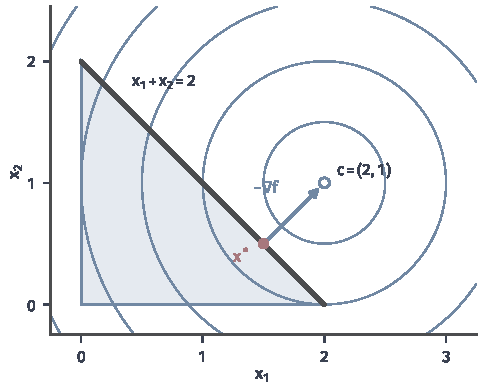
\includegraphics[width=82mm]{figures/05-optimization/06-constrained-optimization/matplotlib/kkt-budget-boundary/figure.pdf}
  \caption{预算分配（$\tau=2$）的边界最优点。浅蓝三角形是可行集，蓝色圆是目标$\frac12\lVert\bm{x}-\bm{c}\rVert_2^2$的等高线，空心点是不可行的理想分配$\bm{c}=(2,1)$，深灰粗线是起作用的预算线。红点$\bm{x}^\star=(3/2,1/2)$处，负梯度（蓝色箭头）非零，指向可行集外。}
  \label{fig:kkt-budget-boundary}
\end{BookInlineFigure}

\paragraph{一般形式}
本章和本部分后面各章都讨论下面的问题。给定$\bm{x}\in\mathbb{R}^n$的目标函数$f$、不等式约束函数$g_1,\ldots,g_m$和等式约束函数$h_1,\ldots,h_p$，求解
\begin{equation}
 \begin{aligned}
  \min_{\bm{x}\in\mathbb{R}^n}\quad&f(\bm{x})\\
  \text{s.t.}\quad&g_i(\bm{x})\leq0,\quad i=1,\ldots,m,\\
  &h_j(\bm{x})=0,\quad j=1,\ldots,p.
 \end{aligned}
 \label{eq:kkt-problem}
\end{equation}
可行集记为
\begin{equation}
 \bm{C}=\{\bm{x}\in\mathbb{R}^n:g_i(\bm{x})\leq0,\ i=1,\ldots,m;\ h_j(\bm{x})=0,\ j=1,\ldots,p\}.
 \label{eq:kkt-feasible}
\end{equation}

除非另有说明，假设$f$、$g_i$、$h_j$都定义在包含$\bm{C}$的开集上，并且连续可微；讨论二阶条件时再要求二阶连续可微。所有不等式都整理成“$\leq0$”，这个约定决定了后面乘子的符号。预算分配写成这种形式，三个不等式约束是
\begin{equation}
 g_1(\bm{x})=x_1+x_2-\tau,\qquad g_2(\bm{x})=-x_1,\qquad g_3(\bm{x})=-x_2.
 \label{eq:kkt-budget-constraints}
\end{equation}
它们的梯度依次是常向量$(1,1)$、$(-1,0)$、$(0,-1)$，都指向使约束函数增大的一侧，也就是可行集的外侧。

\paragraph{活动约束}
站在一个可行点$\bar{\bm{x}}$上，不等式约束分成两类。若$g_i(\bar{\bm{x}})=0$，这条约束正好卡在边界上，稍有不慎就会违反，称它在$\bar{\bm{x}}$处是\term{活动约束}（active constraint）。若$g_i(\bar{\bm{x}})<0$，$g_i$是连续函数，所以在$\bar{\bm{x}}$的某个邻域内仍有$g_i<0$，这条约束在局部不起任何限制作用。活动约束的下标集记为
\begin{equation}
 A(\bar{\bm{x}})=\{i\in\{1,\ldots,m\}:g_i(\bar{\bm{x}})=0\},
 \label{eq:kkt-active-set}
\end{equation}
称为\term{活动集}（active set）。等式约束总在起作用，但$A(\bar{\bm{x}})$只记不等式的下标。

图~\ref{fig:kkt-active-sets}取$\tau=2$，看三个可行点。内部点$(0.6,0.6)$没有活动约束，四周都能走。预算线上的点$(3/2,1/2)$只有$g_1$活动，能走的方向少了一半。角点$(2,0)$处$g_1$与$g_3$同时活动，能走的方向只剩一个楔形。虚线圆是一个小邻域，圆内真正影响移动的只有粗线。

\begin{BookInlineFigure}
  \centering
  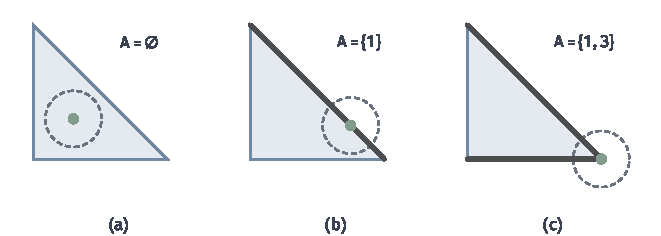
\includegraphics[width=112mm]{figures/05-optimization/06-constrained-optimization/matplotlib/kkt-active-sets/figure.pdf}
  \caption{预算三角形（$\tau=2$）中三个可行点的活动集。深灰粗线是该点的活动约束，虚线圆是一个小邻域。(a)内部点$(0.6,0.6)$没有活动约束。(b)预算线上的点$(3/2,1/2)$只有$g_1$活动。(c)角点$(2,0)$处$g_1$、$g_3$同时活动。}
  \label{fig:kkt-active-sets}
\end{BookInlineFigure}

\paragraph{局部与全局最小点}
第~\ref{chap:optimization}章区分了局部与全局最优解，本章沿用这两个概念，并按习惯称最优解为最小点。称可行点$\bm{x}^\star$是\term{局部最小点}（local minimizer），如果存在$r>0$，使
\begin{equation}
 f(\bm{x}^\star)\leq f(\bm{x})\quad\text{对所有}\ \bm{x}\in\bm{C},\ \lVert\bm{x}-\bm{x}^\star\rVert_2<r.
 \label{eq:kkt-local-min}
\end{equation}
若对$\bm{x}\neq\bm{x}^\star$不等式都严格成立，就称为严格局部最小点。要是式~\eqref{eq:kkt-local-min}对所有$\bm{x}\in\bm{C}$成立，$\bm{x}^\star$就是全局最小点。

比较只在可行点之间进行，所以邻域外和可行集外的点都不参加比较。下面的例子可以看出局部和全局的差别，而这两种点都可以落在边界上。在平面上最小化$f(\bm{x})=x_1$，约束是
\[
 g(\bm{x})=(x_2^2-1)^2+0.3\,x_2-x_1\leq0.
\]
可行集的左边界是一条弯曲的曲线，它有两个向左伸的凸起。

图~\ref{fig:kkt-local-global}中，每个凸起的顶点都比附近的可行点更靠左，因此都是局部最小点。解一元方程求边界曲线的极小，得到上方顶点约为$(0.294,0.960)$，下方顶点约为$(-0.305,-1.036)$，后者才是全局最小点。两处的梯度都等于$(1,0)$，并不为零。站在局部最小点上，只看附近无从知道下方还有更低的点，所以局部信息最多只能回答局部问题。

\begin{BookInlineFigure}
  \centering
  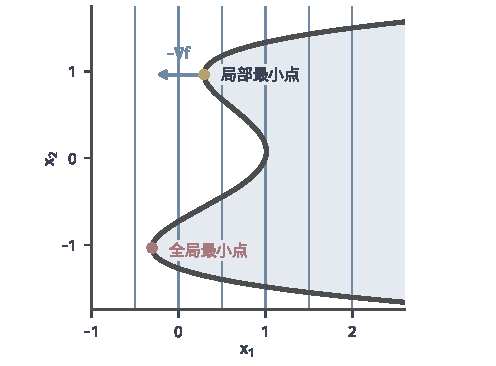
\includegraphics[width=84mm]{figures/05-optimization/06-constrained-optimization/matplotlib/kkt-local-global/figure.pdf}
  \caption{边界上的局部最小点与全局最小点。目标$f(\bm{x})=x_1$的等高线是竖直的蓝线，浅蓝区域是可行集$x_1\geq(x_2^2-1)^2+0.3x_2$，深灰粗线是边界。黄点是局部最小点，红点是全局最小点，两点的负梯度（蓝色箭头）都指向可行集外。}
  \label{fig:kkt-local-global}
\end{BookInlineFigure}

判断最优性时，本章要回答三个不同的问题：局部最小点必须满足什么（必要条件）？满足什么就一定是局部最小点（局部充分条件）？什么时候局部信息足以断定全局最优？解的存在性由第~\ref{chap:optimization}章的结论负责，例如预算三角形是非空紧集，目标连续，最优解一定存在。

\section{可行变化}
\label{sec:kkt-variations}

无约束时，最优性的论证是沿每个方向走一小步，目标都不能下降。有了约束，问题变成：站在候选点上，究竟可以朝哪些方向移动？本节先只看可行集合本身回答这个问题，再看约束函数给出的线性近似，并比较两者。这两个对象不同：前者是真实能走的方向，后者是约束函数在一阶意义下允许的方向。

\subsection{直线移动与切锥}
\label{sec:kkt-tangent-cone}

\paragraph{沿直线可行}
第~\ref{chap:optimization}章已经定义了可行方向：若$t>0$充分小时$\bar{\bm{x}}+t\bm{d}\in\bm{C}$，就称$\bm{d}$是$\bar{\bm{x}}$处的可行方向。可行集凸的时候，这个概念够用。任取$\bm{y}\in\bm{C}$，线段$\bar{\bm{x}}+t(\bm{y}-\bar{\bm{x}})$（$0\leq t\leq1$）都在$\bm{C}$里，所以每个$\bm{y}-\bar{\bm{x}}$都是可行方向，如图~\ref{fig:kkt-line-vs-arc}(a)。

\begin{BookInlineFigure}
  \centering
  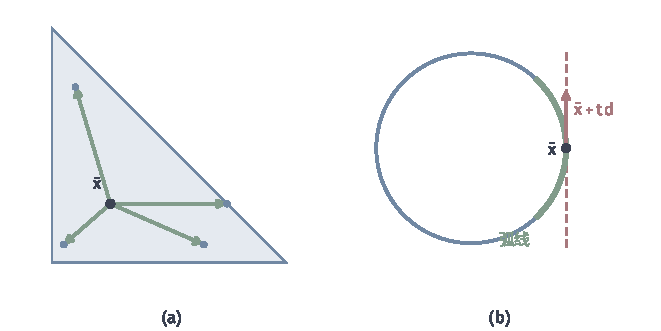
\includegraphics[width=112mm]{figures/05-optimization/06-constrained-optimization/matplotlib/kkt-line-vs-arc/figure.pdf}
  \caption{直线移动与弧线移动。(a)凸集中，从$\bar{\bm{x}}$到任意可行点的线段（绿色箭头）都留在集合内。(b)可行集是单位圆周（蓝线）。从$\bar{\bm{x}}=(1,0)$沿切线走的红色直线立刻离开圆周，而绿色弧线一直可行，并且在$\bar{\bm{x}}$处与直线相切。}
  \label{fig:kkt-line-vs-arc}
\end{BookInlineFigure}

可行集弯曲时，这个定义就不够用了。设$\bm{C}$是单位圆周，也就是$h(\bm{x})=x_1^2+x_2^2-1=0$的解集，取$\bar{\bm{x}}=(1,0)$。若$\bar{\bm{x}}+t\bm{d}$对小的$t>0$都在圆周上，展开$h$并除以$t$，得到
\[
 2d_1+t\lVert\bm{d}\rVert_2^2=0\quad\text{对所有充分小的}\ t>0.
\]
令$t$取两个不同的值，两式相减得$\lVert\bm{d}\rVert_2=0$。所以除零方向外没有可行方向。

可是点明明能沿圆周移动，图~\ref{fig:kkt-line-vs-arc}(b)的绿色弧线就是这样的移动。直线走不通，弧线走得通，弧线在出发时的速度方向是$(0,1)$。因此“能走的方向”不应理解成沿直线可行，而应理解成沿某条可行路径出发的速度。

\paragraph{用放大镜定义方向}
为了把这个想法写成定义，可以想象拿放大镜对准$\bar{\bm{x}}$看可行集。放大倍数越高，圆弧看起来越直，极限是一条直线。写成算式，就是取趋于$\bar{\bm{x}}$的可行点列，把位移除以一个趋于零的正数，看它的极限。

\begin{definition}[切锥]
\label{def:kkt-tangent-cone}
设$\bm{C}\subseteq\mathbb{R}^n$，$\bar{\bm{x}}\in\bm{C}$。称$\bm{d}\in\mathbb{R}^n$是$\bm{C}$在$\bar{\bm{x}}$处的切向量，如果存在可行点列$\bm{x}^{(k)}\in\bm{C}$与正数列$t_k$，使$\bm{x}^{(k)}\to\bar{\bm{x}}$，$t_k\downarrow0$，并且
\begin{equation}
 \frac{\bm{x}^{(k)}-\bar{\bm{x}}}{t_k}\to\bm{d}.
 \label{eq:kkt-tangent-limit}
\end{equation}
全体切向量组成的集合称为\term{切锥}（tangent cone），记为$\bm{T}_{\bm{C}}(\bar{\bm{x}})$。
\end{definition}

上标$(k)$是点列编号，不表示算法迭代。这里$1/t_k$就是放大倍数，点列可以是沿曲线取的点，也可以是在集合中跳跃着逼近的点。沿固定直线可行的方向一定是切向量：取$\bm{x}^{(k)}=\bar{\bm{x}}+t_k\bm{d}$即可。反过来不成立，圆周就是反例。

下面在圆周上走一遍定义。取$t_k=2^{-(k-1)}$，$\bm{x}^{(k)}=(\cos t_k,\sin t_k)$，放大后的位移是
\[
 \frac{\bm{x}^{(k)}-\bar{\bm{x}}}{t_k}=\Bigl(\frac{\cos t_k-1}{t_k},\frac{\sin t_k}{t_k}\Bigr).
\]
前三项依次约为$(-0.460,0.841)$、$(-0.245,0.959)$、$(-0.124,0.990)$，极限是$(0,1)$。

图~\ref{fig:kkt-tangent-sequence}左边是原始尺度下的割线，它们越来越贴近圆弧；右边是放大后的位移，绿色箭头收拢到红色的$(0,1)$。换成$t_k/s$（$s>0$）作分母，极限变成$s(0,1)$；沿圆周的另一侧取点，得到$-s(0,1)$。所以切锥至少包含整条竖直直线。下一小节会用约束函数证明切锥恰好就是这条直线。

\begin{BookInlineFigure}
  \centering
  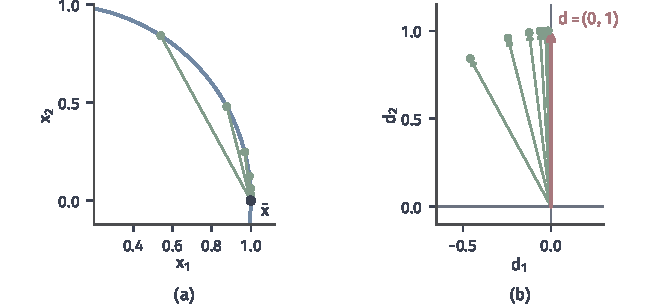
\includegraphics[width=112mm]{figures/05-optimization/06-constrained-optimization/matplotlib/kkt-tangent-sequence/figure.pdf}
  \caption{切向量是放大后位移的极限。可行集为单位圆周，$\bar{\bm{x}}=(1,0)$，$t_k=2^{-(k-1)}$（$k=1,\ldots,6$）。(a)绿点是$\bm{x}^{(k)}=(\cos t_k,\sin t_k)$，绿线是割线。(b)绿色箭头是$(\bm{x}^{(k)}-\bar{\bm{x}})/t_k$，它们趋于红色箭头$\bm{d}=(0,1)$。}
  \label{fig:kkt-tangent-sequence}
\end{BookInlineFigure}

\paragraph{切锥的基本性质}
后面的证明要用到切锥的两条性质，第二条尤其重要，它允许我们用切向量的极限产生新的切向量。

\begin{lemma}[切锥是闭锥]
\label{lem:kkt-tangent-closed}
$\bm{T}_{\bm{C}}(\bar{\bm{x}})$包含零向量，对正数倍封闭，并且是闭集。
\end{lemma}

\begin{proof}
取$\bm{x}^{(k)}=\bar{\bm{x}}$就得到零向量。若$\bm{d}$对应$(\bm{x}^{(k)},t_k)$，$s>0$，则同一点列配$t_k/s$给出$s\bm{d}$。

再证闭性。设切向量列$\bm{d}_l\to\bm{d}$。对每个$l$，由定义可以在$\bm{d}_l$对应的点列中取一项，得到可行点$\bm{y}_l$和正数$\epsilon_l<1/l$，使
\[
 \lVert\bm{y}_l-\bar{\bm{x}}\rVert_2\leq\frac1l,\qquad
 \Bigl\lVert\frac{\bm{y}_l-\bar{\bm{x}}}{\epsilon_l}-\bm{d}_l\Bigr\rVert_2\leq\frac1l.
\]
令$l\to\infty$，有$\bm{y}_l\to\bar{\bm{x}}$，$\epsilon_l\to0$（必要时取子列使$\epsilon_l$单调递减），位移比趋于$\bm{d}$。所以$\bm{d}$是切向量。
\end{proof}

图~\ref{fig:kkt-tangent-cones}是几种常见的形状。内点处四周都能走，切锥是全空间。光滑边界上，放大后边界变成直线，切锥是半空间。角点处切锥是楔形。尖点处两条边界相切，放大后楔形被压成一条线，切锥只剩一条射线。

\begin{BookInlineFigure}
  \centering
  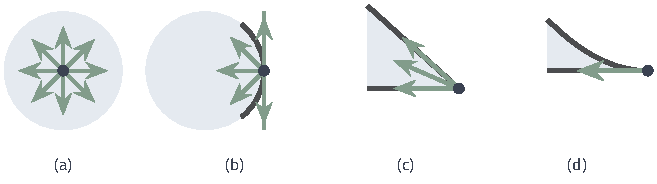
\includegraphics[width=111.3mm]{figures/05-optimization/06-constrained-optimization/tikz/kkt-tangent-cones/figure.pdf}
  \caption{切锥的四种形状。浅蓝区域是可行集，黑点是基点，绿色箭头表示切向量，深灰粗线是边界。(a)内点：全部方向。(b)光滑边界：半空间，边界上的绿线是它的分界。(c)角点：楔形。(d)尖点：只有一条射线。}
  \label{fig:kkt-tangent-cones}
\end{BookInlineFigure}

切锥未必是凸集。集合$\{\bm{x}:x_1x_2=0\}$由两条坐标轴组成，它在原点的切锥就是这两条坐标轴本身。名字里的“锥”只表示对正数倍封闭。

\subsection{一阶必要条件}
\label{sec:kkt-first-order}

现在可以回答：局部最小点在切向量上要满足什么？直观上，沿任何可行路径出发，目标都不能以一阶速度下降。把路径换成切锥定义中的点列，证明只需要一次Taylor展开。

\begin{theorem}[切锥上的一阶必要条件]
\label{thm:kkt-tangent-necessary}
设$\bm{x}^\star$是$f$在$\bm{C}$上的局部最小点，$f$在$\bm{x}^\star$处可微。则
\begin{equation}
 \langle\nabla f(\bm{x}^\star),\bm{d}\rangle\geq0\quad\text{对所有}\ \bm{d}\in\bm{T}_{\bm{C}}(\bm{x}^\star).
 \label{eq:kkt-tangent-necessary}
\end{equation}
\end{theorem}

\begin{proof}
取切向量$\bm{d}$及相应的$\bm{x}^{(k)}$、$t_k$，记位移$\bm{u}_k=\bm{x}^{(k)}-\bm{x}^\star$。$f$在$\bm{x}^\star$处可微，所以
\[
 f(\bm{x}^{(k)})-f(\bm{x}^\star)=\langle\nabla f(\bm{x}^\star),\bm{u}_k\rangle+r_k,
 \qquad\frac{r_k}{\lVert\bm{u}_k\rVert_2}\to0,
\]
其中$\bm{u}_k=\bm{0}$时取$r_k=0$，比值按零理解。

$k$充分大时$\bm{x}^{(k)}$落在式~\eqref{eq:kkt-local-min}的邻域内，左端非负。两边除以$t_k$，得到
\[
 0\leq\Bigl\langle\nabla f(\bm{x}^\star),\frac{\bm{u}_k}{t_k}\Bigr\rangle+\frac{r_k}{t_k}.
\]

由$\bm{u}_k/t_k\to\bm{d}$知$\lVert\bm{u}_k\rVert_2/t_k$有界，所以$r_k/t_k\to0$。令$k\to\infty$，即得式~\eqref{eq:kkt-tangent-necessary}。
\end{proof}

在预算例上试用这个条件（$\tau=2$）。先看不是最优的点$\bar{\bm{x}}=(1,1)$，它在预算线上，梯度是$(-1,0)$。沿预算线的切向量$\bm{d}=(1,-1)$有
\[
 \langle\nabla f(\bar{\bm{x}}),\bm{d}\rangle=-1<0.
\]
直接代入也一样：$f(1+s,1-s)=\frac12[(1-s)^2+s^2]$在$s=0$处的导数是$-1$。所以$(1,1)$不是局部最小点。

再看$\bm{x}^\star=(3/2,1/2)$。这里切锥是半平面$\{\bm{d}:d_1+d_2\leq0\}$，梯度是$(-1/2,-1/2)$，于是对切锥中每个$\bm{d}$，
\[
 \langle\nabla f(\bm{x}^\star),\bm{d}\rangle=-\frac12(d_1+d_2)\geq0.
\]
必要条件成立。图~\ref{fig:kkt-first-order-test}比较了这两个点：(a)中负梯度有沿边界的分量，绿色切向量与负梯度成锐角；(b)中负梯度与边界垂直，沿边界两侧移动都没有一阶下降。

\begin{BookInlineFigure}
  \centering
  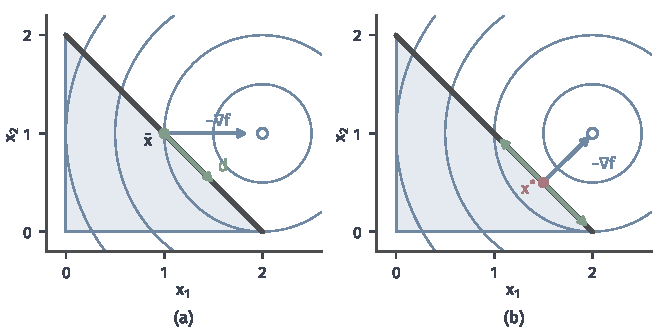
\includegraphics[width=112mm]{figures/05-optimization/06-constrained-optimization/matplotlib/kkt-first-order-test/figure.pdf}
  \caption{切向量上的一阶检验（预算例，$\tau=2$）。空心点是理想分配$\bm{c}$，蓝色箭头是负梯度，绿色箭头是沿预算线的切向量。(a)在$\bar{\bm{x}}=(1,1)$，切向量$\bm{d}=(1,-1)$与负梯度成锐角，目标可以下降。(b)在红点$\bm{x}^\star=(3/2,1/2)$，负梯度垂直于预算线，不存在下降的切向量。}
  \label{fig:kkt-first-order-test}
\end{BookInlineFigure}

\paragraph{凸可行集：法锥}
可行集凸时，每个$\bm{y}-\bm{x}^\star$都是切向量，所以条件可以写成对全部可行点的检验，把切向量这个中间概念拿掉。我们把这个条件从“梯度与所有可行方向的夹角”改写到集合一侧，定义所有“指向集合外”的向量。

\begin{definition}[法锥]
\label{def:kkt-normal-cone}
设$\bm{C}\subseteq\mathbb{R}^n$是凸集，$\bar{\bm{x}}\in\bm{C}$。集合
\begin{equation}
 \bm{N}_{\bm{C}}(\bar{\bm{x}})=\{\bm{v}\in\mathbb{R}^n:\langle\bm{v},\bm{y}-\bar{\bm{x}}\rangle\leq0\ \text{对所有}\ \bm{y}\in\bm{C}\}
 \label{eq:kkt-normal-cone}
\end{equation}
称为$\bm{C}$在$\bar{\bm{x}}$处的\term{法锥}（normal cone）。
\end{definition}

法锥里的向量与所有从$\bar{\bm{x}}$出发的可行弦成钝角或直角，它们都指向集合外侧。负梯度只要落在法锥里，朝可行集内部就没有一阶下降。

\begin{theorem}[凸可行集上的一阶条件]
\label{thm:kkt-convex-set-first-order}
设$\bm{C}$是凸集，$f$在包含$\bm{C}$的开集上可微，$\bm{x}^\star\in\bm{C}$。若$\bm{x}^\star$是$f$在$\bm{C}$上的局部最小点，则
\begin{equation}
 \langle\nabla f(\bm{x}^\star),\bm{y}-\bm{x}^\star\rangle\geq0\quad\text{对所有}\ \bm{y}\in\bm{C},
 \label{eq:kkt-vi}
\end{equation}
等价地，$-\nabla f(\bm{x}^\star)\in\bm{N}_{\bm{C}}(\bm{x}^\star)$。若$f$还在$\bm{C}$上凸，则式~\eqref{eq:kkt-vi}也推出$\bm{x}^\star$是全局最小点。
\end{theorem}

\begin{proof}
必要性：$\bm{y}-\bm{x}^\star$是可行方向，也是切向量，由定理~\ref{thm:kkt-tangent-necessary}得到式~\eqref{eq:kkt-vi}。等价写法只是把$\bm{v}=-\nabla f(\bm{x}^\star)$代入式~\eqref{eq:kkt-normal-cone}。

充分性：取$\bm{y}\in\bm{C}$，$t\in(0,1]$。由$f$的凸性，
\[
 f\bigl(\bm{x}^\star+t(\bm{y}-\bm{x}^\star)\bigr)\leq(1-t)f(\bm{x}^\star)+tf(\bm{y}).
\]
移项，除以$t$，再令$t\downarrow0$，左端的差商趋于方向导数，于是
\[
 \langle\nabla f(\bm{x}^\star),\bm{y}-\bm{x}^\star\rangle\leq f(\bm{y})-f(\bm{x}^\star).
\]
由式~\eqref{eq:kkt-vi}，左端非负，所以$f(\bm{y})\geq f(\bm{x}^\star)$。
\end{proof}

式~\eqref{eq:kkt-vi}称为\term{变分不等式}（variational inequality）。图~\ref{fig:kkt-normal-cones}让预算$\tau$从大变小，法锥依次是三种形状。

$\tau=4$时最优点$\bm{c}=(2,1)$在内部，法锥只有零向量，条件退化为$\nabla f=\bm{0}$。$\tau=2$时最优点在预算线上，法锥是外法向$(1,1)$方向的射线，$-\nabla f=(1/2,1/2)$落在上面。

$\tau=1/2$时，最优点是角点$(1/2,0)$。法锥由两条边的外法向$(1,1)$、$(0,-1)$张成。这一点可以直接核对：设$\bm{v}\in\bm{N}_{\bm{C}}$，用沿两条边的可行弦方向$(-1,1)$与$(-1,0)$代入式~\eqref{eq:kkt-normal-cone}，得到$v_2\leq v_1$与$v_1\geq0$，这恰好说明
\[
 \bm{v}=v_1(1,1)+(v_1-v_2)(0,-1),\qquad v_1\geq0,\ v_1-v_2\geq0.
\]
角点的法锥比边上的法锥大，能接住更多方向的负梯度。

\begin{BookInlineFigure}
  \centering
  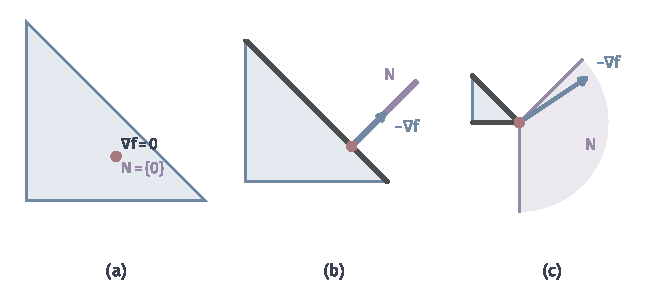
\includegraphics[width=112mm]{figures/05-optimization/06-constrained-optimization/matplotlib/kkt-normal-cones/figure.pdf}
  \caption{预算例中最优点处的法锥（紫色）。红点是最优点，蓝色箭头是负梯度（(c)中按$0.5$倍缩短）。(a)$\tau=4$，最优点在内部，法锥为$\{\bm{0}\}$。(b)$\tau=2$，法锥是一条射线，负梯度落在上面。(c)$\tau=1/2$，最优点是角点，法锥是两条外法向张成的楔形，负梯度落在其中。}
  \label{fig:kkt-normal-cones}
\end{BookInlineFigure}

定理的充分性同时需要可行集与目标都凸。只有目标凸是不够的：在单位圆周上最小化$\frac12\lVert\bm{x}-(2,0)\rVert_2^2$，点$(-1,0)$的梯度是$(-3,0)$，切向量只有$(0,s)$，与梯度垂直，一阶条件成立；可它是圆周上离$(2,0)$最远的点。本章后面还会回到这个例子。

\subsection{约束的线性化}
\label{sec:kkt-linearized}

切锥描述得准，却不好算，我们无法枚举所有点列。约束以函数形式给出时，有一个自然的替代品：在基点把约束函数展开到一阶，看一阶近似允许哪些方向。

设$\bar{\bm{x}}$可行，沿$\bm{d}$走一小步，约束函数近似变化为
\[
 g_i(\bar{\bm{x}}+t\bm{d})\approx g_i(\bar{\bm{x}})+t\langle\nabla g_i(\bar{\bm{x}}),\bm{d}\rangle.
\]
不活动的约束有余量，一阶近似不构成限制。活动约束要求这一项不为正，等式约束要求它等于零。

\begin{definition}[线性化锥]
\label{def:kkt-linearized-cone}
设$\bar{\bm{x}}\in\bm{C}$，约束函数在$\bar{\bm{x}}$处可微。集合
\begin{equation}
 \bm{F}(\bar{\bm{x}})=\left\{\bm{d}\in\mathbb{R}^n:
 \begin{aligned}
  &\langle\nabla h_j(\bar{\bm{x}}),\bm{d}\rangle=0,\ j=1,\ldots,p,\\
  &\langle\nabla g_i(\bar{\bm{x}}),\bm{d}\rangle\leq0,\ i\in A(\bar{\bm{x}})
 \end{aligned}
 \right\}
 \label{eq:kkt-linearized-cone}
\end{equation}
称为$\bar{\bm{x}}$处的\term{线性化锥}（linearized cone）。
\end{definition}

$\bm{F}(\bar{\bm{x}})$是有限个线性不等式的解集，一眼就能写出。例如预算例$\tau=1/2$的角点$(1/2,0)$处，$g_1$和$g_3$活动，于是
\[
 \bm{F}=\{\bm{d}:d_1+d_2\leq0,\ -d_2\leq0\}.
\]
单位圆周在$(1,0)$处，$\nabla h=(2,0)$，于是$\bm{F}=\{\bm{d}:d_1=0\}$，正是前面算出的竖直直线。

真实能走的方向一定通过这个一阶检查，因此切锥总在线性化锥之内。

\begin{theorem}[切锥包含于线性化锥]
\label{thm:kkt-tangent-in-linearized}
设$\bar{\bm{x}}\in\bm{C}$，$g_i$（$i\in A(\bar{\bm{x}})$）与$h_j$在$\bar{\bm{x}}$处可微。则
\begin{equation}
 \bm{T}_{\bm{C}}(\bar{\bm{x}})\subseteq\bm{F}(\bar{\bm{x}}).
 \label{eq:kkt-tangent-in-linearized}
\end{equation}
\end{theorem}

\begin{proof}
取切向量$\bm{d}$及相应的$\bm{x}^{(k)}$、$t_k$，对活动的$g_i$，由可微性，
\[
 g_i(\bm{x}^{(k)})=g_i(\bar{\bm{x}})+\langle\nabla g_i(\bar{\bm{x}}),\bm{x}^{(k)}-\bar{\bm{x}}\rangle+o(\lVert\bm{x}^{(k)}-\bar{\bm{x}}\rVert_2).
\]
这里$g_i(\bar{\bm{x}})=0$，$g_i(\bm{x}^{(k)})\leq0$。除以$t_k$并令$k\to\infty$，余项如定理~\ref{thm:kkt-tangent-necessary}的证明一样趋于零，得到
\[
 \langle\nabla g_i(\bar{\bm{x}}),\bm{d}\rangle\leq0.
\]

对$h_j$同样展开，此时左端恒为零，极限给出$\langle\nabla h_j(\bar{\bm{x}}),\bm{d}\rangle=0$。
\end{proof}

圆周的例子到这里算完了：切锥包含竖直直线，又包含于$\bm{F}=\{\bm{d}:d_1=0\}$，所以它就是这条直线。

式~\eqref{eq:kkt-tangent-in-linearized}可以是严格包含。考虑一维约束$g(x)=x^2\leq0$，可行集只有原点，切锥是$\{0\}$。可是$g'(0)=0$，线性化没有施加任何限制，$\bm{F}(0)=\mathbb{R}$。一阶近似把这条弯曲的约束看成了常值零，图~\ref{fig:kkt-linearization}(b)的黄色线就是这个近似。

\begin{BookInlineFigure}
  \centering
  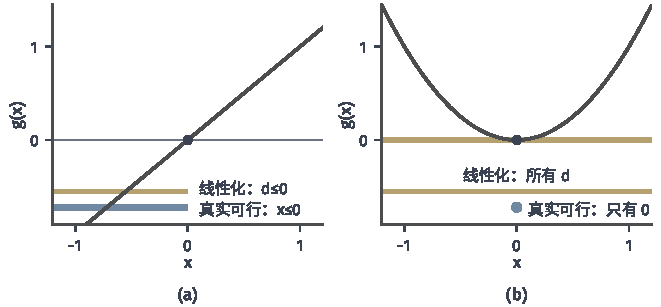
\includegraphics[width=112mm]{figures/05-optimization/06-constrained-optimization/matplotlib/kkt-linearization/figure.pdf}
  \caption{线性化与真实可行集的比较。深灰曲线是$g$，下方黄带是线性化允许的方向，蓝带（点）是真实的可行点。(a)$g(x)=x$，线性化与真实情况一致。(b)$g(x)=x^2$，$g'(0)=0$，切线（黄色）恒为零，线性化允许所有方向，而可行集只有原点。}
  \label{fig:kkt-linearization}
\end{BookInlineFigure}

二维的例子能看得更清楚。取$g_1(\bm{x})=x_2-(1-x_1)^3\leq0$，$g_2(\bm{x})=-x_2\leq0$，点$\bar{\bm{x}}=(1,0)$，两条约束都活动。可行点要满足$0\leq x_2\leq(1-x_1)^3$，所以$x_1\leq1$，可行集在$\bar{\bm{x}}$处形成一个向右的尖点。

梯度分别是$(0,1)$和$(0,-1)$，线性化要求$d_2\leq0$且$-d_2\leq0$，即$d_2=0$，于是
\[
 \bm{F}(\bar{\bm{x}})=\{\bm{d}:d_2=0\},\qquad
 \bm{T}_{\bm{C}}(\bar{\bm{x}})=\{(-s,0):s\geq0\}.
\]
线性化多出了向右的半条直线。图~\ref{fig:kkt-cusp}中的红色箭头就是虚假方向：若最小化$f(\bm{x})=-x_1$，$\bar{\bm{x}}$是全局最小点，而$\bm{d}=(1,0)$在线性化下“可行”，并使$\langle\nabla f,\bm{d}\rangle=-1<0$。只看线性化，就会误以为还能下降。

\begin{BookInlineFigure}
  \centering
  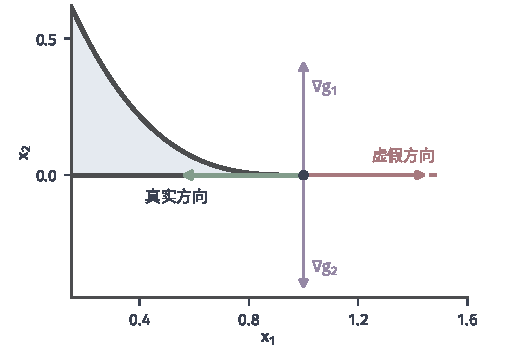
\includegraphics[width=88mm]{figures/05-optimization/06-constrained-optimization/matplotlib/kkt-cusp/figure.pdf}
  \caption{尖点处线性化引入虚假方向。浅蓝区域是可行集$0\leq x_2\leq(1-x_1)^3$，紫色箭头是两条活动约束的梯度$(0,\pm1)$。线性化只要求$d_2=0$，向左的绿色箭头是真实切向量，向右的红色箭头是虚假方向。}
  \label{fig:kkt-cusp}
\end{BookInlineFigure}

表~\ref{tab:kkt-tangent-vs-linearized}对比这两个对象。下一节要回答的问题由此而来：什么时候两者相等，使我们可以用好算的线性化锥代替真实的切锥？

\begin{BookInlineTable}
  \centering
  \begin{tabular}{@{}lll@{}}
    \toprule
    对比项 & 切锥$\bm{T}_{\bm{C}}$ & 线性化锥$\bm{F}$\\
    \midrule
    依赖什么 & 只依赖集合$\bm{C}$ & 依赖约束函数的写法\\
    含义 & 真实可行变化 & 一阶模型允许的变化\\
    计算 & 一般需要分析点列 & 解线性不等式\\
    关系 & 总包含在$\bm{F}$内 & 可能多出虚假方向\\
    \bottomrule
  \end{tabular}
  \caption{切锥与线性化锥的比较。}
  \label{tab:kkt-tangent-vs-linearized}
\end{BookInlineTable}

\section{约束资格}
\label{sec:kkt-cq}

定理~\ref{thm:kkt-tangent-necessary}是关于切锥的，而能算的是线性化锥。两者之间差一个包含关系。本节研究：约束函数在一点满足什么条件，线性化就没有引入虚假方向，也就是切锥等于线性化锥？这类只涉及约束函数、不涉及目标的条件称为\term{约束资格}（constraint qualification）。

约束资格和凸性是两回事。约束$x^2\leq0$是凸函数，问题也可以是凸的，但它的线性化在原点失效。反过来，圆周这样的非凸集合，线性化却是准确的。约束资格检查的是约束函数在这一点的一阶信息够不够用，和目标函数是否凸没有关系。

\subsection{线性无关约束资格}
\label{sec:kkt-licq}

先看线性化为什么可能准确。在圆周的$(1,0)$处，沿切线走一步$(1,t)$会离开圆周，但偏离只有$t$的二阶小量，沿圆的法向拉回去一点，就回到圆周上。拉回动作所需的修正量比$t$小得多，放大看不出来，所以切线方向是真实可行的。

这个拉回动作要能实施，需要约束的梯度在拉回的方向上足够“有劲”，也就是各约束可以被独立地修正。这就是下面的条件。

\begin{definition}[线性无关约束资格]
\label{def:kkt-licq}
设$\bar{\bm{x}}\in\bm{C}$。若向量组
\begin{equation}
 \{\nabla h_j(\bar{\bm{x}}):j=1,\ldots,p\}\cup\{\nabla g_i(\bar{\bm{x}}):i\in A(\bar{\bm{x}})\}
 \label{eq:kkt-licq}
\end{equation}
线性无关，就称$\bar{\bm{x}}$满足\term{线性无关约束资格}（linear independence constraint qualification，LICQ）。
\end{definition}

图~\ref{fig:kkt-licq-representation}(a)是预算例的角点，梯度$(1,1)$和$(0,-1)$线性无关，LICQ成立。图(c)是上一节的尖点，两个活动梯度共线，LICQ不成立。圆周上$\nabla h=(2x_1,2x_2)$处处非零，单个非零向量线性无关，LICQ处处成立。约束$x^2\leq0$在原点的梯度为零，LICQ不成立。

\begin{BookInlineFigure}
  \centering
  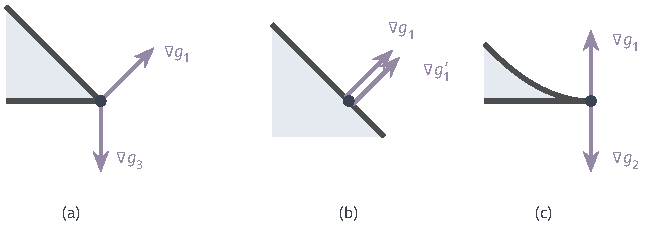
\includegraphics[width=110.3mm]{figures/05-optimization/06-constrained-optimization/tikz/kkt-licq-representation/figure.pdf}
  \caption{活动约束的梯度是否线性无关（紫色箭头）。(a)角点处两条梯度线性无关，LICQ成立。(b)同一条约束写两次，可行集不变，但两个梯度相同（为看清而错开绘制），LICQ不成立。(c)尖点处两个梯度方向相反，LICQ不成立。}
  \label{fig:kkt-licq-representation}
\end{BookInlineFigure}

下面的引理把“拉回”写成隐函数定理的一次应用，它产生一条真正可行的曲线。第~\ref{sec:kkt-second-order}节的二阶必要条件还要用这条曲线。隐函数定理说：方程关于待解变量的Jacobian可逆时，方程在局部确定唯一的连续可微解，详见\BookChapterRef{chap:implicit-inverse-functions}{卷二第22章“隐函数与反函数”}。

\begin{lemma}[沿线性化方向的可行曲线]
\label{lem:kkt-feasible-curve}
设约束函数在$\bar{\bm{x}}\in\bm{C}$附近连续可微，$\bm{d}\in\bm{F}(\bar{\bm{x}})$。设$W\subseteq A(\bar{\bm{x}})$满足：$i\in W$时$\langle\nabla g_i(\bar{\bm{x}}),\bm{d}\rangle=0$，$i\in A(\bar{\bm{x}})\setminus W$时$\langle\nabla g_i(\bar{\bm{x}}),\bm{d}\rangle<0$，并且$\nabla h_j(\bar{\bm{x}})$（全部$j$）与$\nabla g_i(\bar{\bm{x}})$（$i\in W$）线性无关。则存在$\delta>0$和连续可微曲线$\bm{x}:(-\delta,\delta)\to\mathbb{R}^n$，满足
\begin{equation}
 \bm{x}(0)=\bar{\bm{x}},\qquad\bm{x}'(0)=\bm{d},\qquad\bm{x}(t)\in\bm{C}\ \ (0\leq t<\delta),
 \label{eq:kkt-feasible-curve}
\end{equation}
并且$h_j(\bm{x}(t))=0$，$g_i(\bm{x}(t))=0$（$i\in W$）对$\lvert t\rvert<\delta$成立。若约束函数还二阶连续可微，则曲线也二阶连续可微。
\end{lemma}

\begin{proof}
把$h_j$（全部$j$）和$g_i$（$i\in W$）合成向量值函数$\bm{c}$，记它在$\bar{\bm{x}}$处的Jacobian为$\bm{J}\in\mathbb{R}^{r\times n}$。由假设，$\bm{J}$行满秩，$\bm{J}\bm{d}=\bm{0}$。考虑关于$\bm{w}\in\mathbb{R}^r$的方程
\[
 \Phi(t,\bm{w})=\bm{c}(\bar{\bm{x}}+t\bm{d}+\bm{J}^\top\bm{w})=\bm{0}.
\]
这里$\bar{\bm{x}}+t\bm{d}$是沿切线走，$\bm{J}^\top\bm{w}$是沿约束法向的修正。

$\Phi(0,\bm{0})=\bm{0}$，关于$\bm{w}$的Jacobian在该点是$\bm{J}\bm{J}^\top$，行满秩保证它可逆。由隐函数定理，存在连续可微的$\bm{w}(t)$（$\lvert t\rvert<\delta$），$\bm{w}(0)=\bm{0}$，$\Phi(t,\bm{w}(t))=\bm{0}$。隐函数的导数公式给出
\[
 \bm{w}'(0)=-(\bm{J}\bm{J}^\top)^{-1}\bm{J}\bm{d}=\bm{0}.
\]

令
\[
 \bm{x}(t)=\bar{\bm{x}}+t\bm{d}+\bm{J}^\top\bm{w}(t),
\]
于是$\bm{x}'(0)=\bm{d}$，且$\bm{c}(\bm{x}(t))=\bm{0}$。剩下的约束分两类检查。对$i\in A(\bar{\bm{x}})\setminus W$，有
\[
 g_i(\bm{x}(t))=t\langle\nabla g_i(\bar{\bm{x}}),\bm{d}\rangle+o(t),
\]
小的$t>0$时为负。对$i\notin A(\bar{\bm{x}})$，$g_i(\bar{\bm{x}})<0$，由连续性在小$t$时仍为负。缩小$\delta$后，$\bm{x}(t)$在$0\leq t<\delta$时可行。

约束函数二阶连续可微时，隐函数的导数公式
\[
 \bm{w}'(t)=-\bigl[\bm{D}_{\bm{w}}\Phi(t,\bm{w}(t))\bigr]^{-1}\bm{D}_t\Phi(t,\bm{w}(t))
\]
的右端沿解连续可微，所以$\bm{w}$二阶连续可微，曲线也是。
\end{proof}

圆周上可以把这个构造完全算出来。$\bar{\bm{x}}=(1,0)$，$\bm{d}=(0,1)$，$\bm{J}=(2,0)$，修正方程是
\[
 (1+2w)^2+t^2=1.
\]
取$w(0)=0$的解支，得到
\[
 w(t)=\frac{\sqrt{1-t^2}-1}{2}=-\frac{t^2}{4}+o(t^2),\qquad\bm{x}(t)=\bigl(\sqrt{1-t^2},\,t\bigr).
\]
修正量$w$是$t$的二阶小量，这正是$w'(0)=0$的含义。图~\ref{fig:kkt-licq-correction}画出$t=0.3,0.55,0.8$时的切线步和修正，修正量随$t$减小而更快地消失。

\begin{BookInlineFigure}
  \centering
  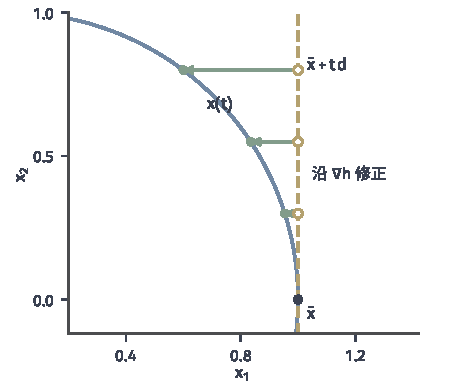
\includegraphics[width=78mm]{figures/05-optimization/06-constrained-optimization/matplotlib/kkt-licq-correction/figure.pdf}
  \caption{用隐函数定理修正线性化方向。蓝线是单位圆周，黄色虚线是切线$\bar{\bm{x}}+t\bm{d}$，黄色空心点是不可行的试探点。绿色箭头沿$\nabla h(\bar{\bm{x}})$方向把试探点拉回圆周，绿点组成可行曲线$\bm{x}(t)$。$t$越小，修正量相对$t$越小。}
  \label{fig:kkt-licq-correction}
\end{BookInlineFigure}

有了可行曲线，线性化方向就全部是真实方向。

\begin{theorem}[LICQ下线性化准确]
\label{thm:kkt-licq-exact}
设约束函数在$\bar{\bm{x}}\in\bm{C}$附近连续可微，$\bar{\bm{x}}$满足LICQ。则
\begin{equation}
 \bm{T}_{\bm{C}}(\bar{\bm{x}})=\bm{F}(\bar{\bm{x}}).
 \label{eq:kkt-licq-exact}
\end{equation}
\end{theorem}

\begin{proof}
包含$\subseteq$是定理~\ref{thm:kkt-tangent-in-linearized}。反过来取$\bm{d}\in\bm{F}(\bar{\bm{x}})$，令
\[
 W=\{i\in A(\bar{\bm{x}}):\langle\nabla g_i(\bar{\bm{x}}),\bm{d}\rangle=0\}.
\]
LICQ保证引理~\ref{lem:kkt-feasible-curve}的线性无关假设成立，得到可行曲线。取$t_k=\delta/(k+1)$，$\bm{x}^{(k)}=\bm{x}(t_k)$，由$\bm{x}'(0)=\bm{d}$知式~\eqref{eq:kkt-tangent-limit}成立，所以$\bm{d}$是切向量。
\end{proof}

\paragraph{条件与约束的写法有关}
LICQ是对约束函数的要求，不是对集合的要求。把预算约束$x_1+x_2\leq\tau$写两遍，可行集一点没变，切锥也没变，但活动梯度$(1,1)$出现两次，线性相关，LICQ就不成立了，见图~\ref{fig:kkt-licq-representation}(b)。这说明LICQ可以因为写法上的冗余而失败，并不代表集合本身有什么毛病。下一小节的条件能容忍这种冗余。

\subsection{Mangasarian--Fromovitz条件}
\label{sec:kkt-mfcq}

回头看证明，线性化准确真正需要什么？对活动不等式来说，严格向内的方向不必拉回，因为它们本来就有一阶余量。只有等式约束要靠拉回来保持。所以只需要等式约束可以被独立修正，并且存在一个同时严格改善所有活动不等式的方向。

\begin{definition}[Mangasarian--Fromovitz约束资格]
\label{def:kkt-mfcq}
设$\bar{\bm{x}}\in\bm{C}$。若$\nabla h_j(\bar{\bm{x}})$（$j=1,\ldots,p$）线性无关，并且存在$\bar{\bm{d}}\in\mathbb{R}^n$，使
\begin{equation}
 \begin{aligned}
  \langle\nabla h_j(\bar{\bm{x}}),\bar{\bm{d}}\rangle&=0,\quad j=1,\ldots,p,\\
  \langle\nabla g_i(\bar{\bm{x}}),\bar{\bm{d}}\rangle&<0,\quad i\in A(\bar{\bm{x}}),
 \end{aligned}
 \label{eq:kkt-mfcq}
\end{equation}
就称$\bar{\bm{x}}$满足\term{Mangasarian--Fromovitz约束资格}（Mangasarian--Fromovitz constraint qualification，MFCQ）。
\end{definition}

条件的两部分各有用途：等式梯度线性无关让我们能用隐函数定理保持等式；方向$\bar{\bm{d}}$让我们能严格走进不等式的内部。图~\ref{fig:kkt-mfcq-direction}(a)中三条活动梯度在平面内必然线性相关，LICQ不成立，但它们都落在某个开半平面内，绿色的$\bar{\bm{d}}$同时与三者成钝角，MFCQ成立。图(b)是尖点：要求$\bar{d}_2<0$与$-\bar{d}_2<0$，两个开半平面不相交，这样的方向不存在。

\begin{BookInlineFigure}
  \centering
  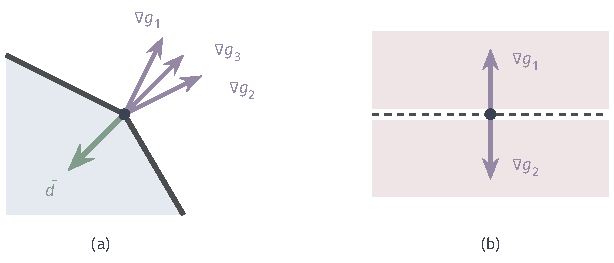
\includegraphics[width=103.9mm]{figures/05-optimization/06-constrained-optimization/tikz/kkt-mfcq-direction/figure.pdf}
  \caption{MFCQ要求存在严格向内的方向。(a)三条活动约束的梯度（紫色）线性相关，但绿色方向$\bar{\bm{d}}$与三者都成钝角，MFCQ成立。(b)两个活动梯度方向相反，使约束严格减小的方向分别在上下两个开半平面（浅红）里，两者不相交，MFCQ不成立。}
  \label{fig:kkt-mfcq-direction}
\end{BookInlineFigure}

两个条件之间有蕴含关系，但不等价。

\begin{lemma}[LICQ蕴含MFCQ]
\label{lem:kkt-licq-implies-mfcq}
若$\bar{\bm{x}}$满足LICQ，则$\bar{\bm{x}}$满足MFCQ。
\end{lemma}

\begin{proof}
以$\nabla h_j(\bar{\bm{x}})$和活动的$\nabla g_i(\bar{\bm{x}})$作行组成矩阵$\bm{J}$，LICQ说明$\bm{J}$行满秩，所以$\bm{J}\bm{J}^\top$可逆。令$\bm{b}$是等式对应分量为$0$、不等式对应分量为$-1$的向量，取
\[
 \bar{\bm{d}}=\bm{J}^\top(\bm{J}\bm{J}^\top)^{-1}\bm{b},
\]
则$\bm{J}\bar{\bm{d}}=\bm{b}$，这正是式~\eqref{eq:kkt-mfcq}。等式梯度作为线性无关组的子集仍线性无关。
\end{proof}

反向不成立。把预算约束写两遍，活动梯度是两个$(1,1)$，LICQ失败；取$\bar{\bm{d}}=(-1,-1)$，内积都是$-2<0$，MFCQ成立。

\begin{theorem}[MFCQ下线性化准确]
\label{thm:kkt-mfcq-exact}
设约束函数在$\bar{\bm{x}}\in\bm{C}$附近连续可微，$\bar{\bm{x}}$满足MFCQ。则式~\eqref{eq:kkt-licq-exact}成立。
\end{theorem}

\begin{proof}
只需证$\bm{F}\subseteq\bm{T}_{\bm{C}}$。取$\bm{d}\in\bm{F}(\bar{\bm{x}})$，对$\epsilon>0$令$\bm{d}_\epsilon=\bm{d}+\epsilon\bar{\bm{d}}$。由式~\eqref{eq:kkt-mfcq}，
\[
 \langle\nabla h_j(\bar{\bm{x}}),\bm{d}_\epsilon\rangle=0,\qquad
 \langle\nabla g_i(\bar{\bm{x}}),\bm{d}_\epsilon\rangle<0,\quad i\in A(\bar{\bm{x}}).
\]

取$W=\varnothing$，引理~\ref{lem:kkt-feasible-curve}的线性无关假设此时只要求等式梯度线性无关，这由MFCQ保证。于是沿$\bm{d}_\epsilon$有可行曲线，$\bm{d}_\epsilon\in\bm{T}_{\bm{C}}(\bar{\bm{x}})$。由引理~\ref{lem:kkt-tangent-closed}，切锥闭，令$\epsilon\downarrow0$得到$\bm{d}\in\bm{T}_{\bm{C}}(\bar{\bm{x}})$。
\end{proof}

这里“先扰动成严格方向，再取极限”这一步是MFCQ证明的关键，它绕开了LICQ需要的全部活动梯度线性无关。

\paragraph{仿射约束与条件的边界}
还有一类不需要任何检查的约束：若全部活动约束和等式约束都是仿射函数，$\bm{d}\in\bm{F}(\bar{\bm{x}})$时直接有$\bar{\bm{x}}+t\bm{d}$在小$t>0$下可行，因此$\bm{T}_{\bm{C}}=\bm{F}$。这正是线性规划不需要讨论约束资格的原因。

约束资格是充分条件，不是线性化准确的必要条件。表~\ref{tab:kkt-three-writings}用同一个集合$\{0\}$的三种写法说明这一点。第三行LICQ和MFCQ都不成立，线性化却是准确的，它属于上面的仿射情形。

\begin{BookInlineTable}
  \centering
  \begin{tabular}{@{}llccc@{}}
    \toprule
    约束写法 & $\bm{F}(0)$ & LICQ & MFCQ & $\bm{T}=\bm{F}$\\
    \midrule
    $x=0$ & $\{0\}$ & 成立 & 成立 & 是\\
    $x^2\leq0$ & $\mathbb{R}$ & 不成立 & 不成立 & 否\\
    $x\leq0$，$-x\leq0$ & $\{0\}$ & 不成立 & 不成立 & 是\\
    \bottomrule
  \end{tabular}
  \caption{同一可行集$\{0\}$的三种写法。切锥恒为$\{0\}$，线性化锥与约束资格随写法改变。}
  \label{tab:kkt-three-writings}
\end{BookInlineTable}

全节的结论可以连成一条链：
\[
 \text{LICQ}\ \Longrightarrow\ \text{MFCQ}\ \Longrightarrow\ \bm{T}_{\bm{C}}=\bm{F}.
\]
有了最后这个等式，切锥上的必要条件就可以放到线性化锥上检验，下一节由此得到关于梯度的方程。

\section{乘子条件}
\label{sec:kkt-multipliers}

到目前为止，局部最小点的必要条件是“线性化锥中没有下降方向”，前提是线性化准确。这句话要对无穷多个方向逐一检验，不便于计算。接下来要弄清：怎样把它改写成有限个关于梯度的方程？先看只有等式约束的情形，再加入不等式，最后回答这组方程何时必要、何时充分。

\subsection{等式约束的Lagrange乘子}
\label{sec:kkt-lagrange}

下面的问题足够小，可以用三种办法解，比较它们就能看出乘子从哪里来：
\begin{equation}
 \min_{\bm{x}\in\mathbb{R}^2}\ \frac12(x_1^2+4x_2^2)\quad\text{s.t.}\quad x_1+x_2=1.
 \label{eq:kkt-equality-qp}
\end{equation}

\paragraph{第一种办法：消去约束}
可行集是一条直线，用参数$s$表示为$\bm{x}(s)=(1-s,s)$。把它代入目标，就成了无约束的一元问题：
\[
 \phi(s)=\frac12\bigl[(1-s)^2+4s^2\bigr],\qquad\phi'(s)=5s-1.
\]
令导数为零，得$s=1/5$。于是
\[
 \bm{x}^\star=\Bigl(\frac45,\frac15\Bigr),\qquad f^\star=\frac12\Bigl(\frac{16}{25}+\frac{4}{25}\Bigr)=\frac25.
\]
$\phi''=5>0$，这是一元凸二次函数的最小点，所以$\bm{x}^\star$是全局最小点。

\paragraph{第二种办法：切向导数为零}
由链式法则，$\phi'(s)$就是梯度沿直线方向$\bm{v}=(-1,1)$的方向导数：
\[
 \phi'(s)=\langle\nabla f(\bm{x}(s)),\bm{v}\rangle=-x_1+4x_2.
\]
令它为零，再加上$x_1+x_2=1$，解出同样的点。这说明最优点的条件是：梯度在约束直线的切向上没有分量。

\paragraph{第三种办法：梯度平行于法向}
切向分量为零，就是说梯度垂直于直线，也就是平行于约束的法向$\nabla h=(1,1)$。在$\bm{x}^\star$处，
\[
 \nabla f(\bm{x}^\star)=\Bigl(\frac45,\frac45\Bigr)=\frac45\,\nabla h(\bm{x}^\star).
\]
把这个比例系数写成$-\nu$，关系就成了$\nabla f+\nu\nabla h=\bm{0}$，这里$\nu=-4/5$。这个系数称为\term{Lagrange乘子}（Lagrange multiplier）。

反过来也能从方程解。未知量是$x_1,x_2,\nu$，方程是
\[
 x_1+\nu=0,\qquad 4x_2+\nu=0,\qquad x_1+x_2=1.
\]
前两式给出$x_1=-\nu$，$x_2=-\nu/4$，代入第三式得$-\frac54\nu=1$，于是$\nu=-4/5$，点仍是$(4/5,1/5)$。这个方程组对任意光滑问题都能写出来，不需要先把约束参数化。

图~\ref{fig:kkt-equality-tangency}(a)是这件事的几何。最优点处直线与一条等高线相切，所以两者法向平行。在非最优的可行点$\bar{\bm{x}}=(0.2,0.8)$，梯度$(0.2,3.2)$不垂直于直线，它沿$\bm{v}$的分量给出$\phi'(0.8)=3$，与图(b)中的斜率相同，反向移动（绿色箭头）就能下降。

\begin{BookInlineFigure}
  \centering
  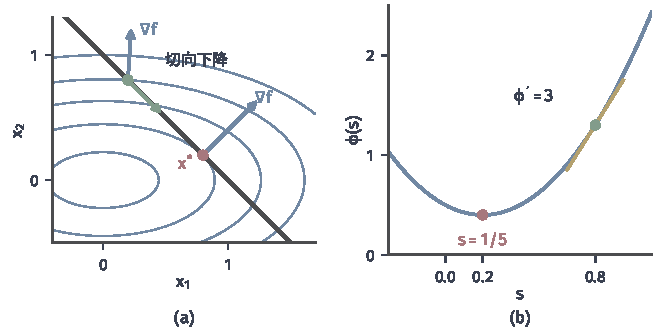
\includegraphics[width=112mm]{figures/05-optimization/06-constrained-optimization/matplotlib/kkt-equality-tangency/figure.pdf}
  \caption{等式约束问题~\eqref{eq:kkt-equality-qp}的切点条件。(a)蓝线是目标的等高线，深灰线是约束直线。红点$\bm{x}^\star=(4/5,1/5)$处直线与等高线相切，梯度沿法向。绿点$(0.2,0.8)$处梯度有切向分量，绿色箭头是沿直线的下降方向。(b)目标沿直线的限制$\phi(s)=f(1-s,s)$，红点是最小点$s=1/5$，绿点$s=0.8$处的切线（黄色）斜率为$3$。}
  \label{fig:kkt-equality-tangency}
\end{BookInlineFigure}

一般的等式约束情形完全一样，只是切向从一条线变成一个子空间。

\begin{theorem}[等式约束的一阶必要条件]
\label{thm:kkt-lagrange}
考虑只有等式约束的问题~\eqref{eq:kkt-problem}（$m=0$）。设$f$、$h_j$在局部最小点$\bm{x}^\star$附近连续可微，$\nabla h_1(\bm{x}^\star),\ldots,\nabla h_p(\bm{x}^\star)$线性无关。则存在唯一的$\bm{\nu}^\star\in\mathbb{R}^p$，使
\begin{equation}
 \nabla f(\bm{x}^\star)+\sum_{j=1}^p\nu_j^\star\nabla h_j(\bm{x}^\star)=\bm{0}.
 \label{eq:kkt-lagrange}
\end{equation}
\end{theorem}

\begin{proof}
以$\nabla h_j(\bm{x}^\star)^\top$为行组成矩阵$\bm{E}$。由定理~\ref{thm:kkt-licq-exact}，切锥等于线性化锥。这里线性化锥就是$\bm{E}$的零空间，是一个子空间。

由定理~\ref{thm:kkt-tangent-necessary}，对这个子空间中的$\bm{d}$有$\langle\nabla f(\bm{x}^\star),\bm{d}\rangle\geq0$。$-\bm{d}$也在子空间内，所以内积只能为零，即$\nabla f(\bm{x}^\star)$与$\bm{E}$的零空间正交。

零空间的正交补是$\bm{E}^\top$的值域，所以存在$\bm{u}$使$\nabla f(\bm{x}^\star)=\bm{E}^\top\bm{u}$，令$\bm{\nu}^\star=-\bm{u}$即得式~\eqref{eq:kkt-lagrange}。唯一性来自$\bm{E}^\top$的列线性无关。
\end{proof}

把目标和约束按乘子加权相加，定义\term{Lagrange函数}（Lagrangian）
\begin{equation}
 \mathcal{L}(\bm{x},\bm{\nu})=f(\bm{x})+\sum_{j=1}^p\nu_jh_j(\bm{x}).
 \label{eq:kkt-lagrangian-equality}
\end{equation}
式~\eqref{eq:kkt-lagrange}就是$\nabla_{\bm{x}}\mathcal{L}=\bm{0}$在$(\bm{x}^\star,\bm{\nu}^\star)$处成立，可行性$h_j=0$就是$\nabla_{\bm{\nu}}\mathcal{L}=\bm{0}$。约束问题的一阶条件由此写成了无约束形式的驻定方程。要注意，这只是驻定，$\mathcal{L}$在$\bm{x}^\star$不必取最小值，更不是在$(\bm{x},\bm{\nu})$上取最小值。

乘子还有一层经济含义。把例子的约束放松成$x_1+x_2=1+\varepsilon$，同样的计算给出最优值$\frac25(1+\varepsilon)^2$，它在$\varepsilon=0$处的导数是$4/5=-\nu$。所以$\lvert\nu\rvert$是约束右端变动一个单位时最优值的变化率，这叫影子价格。这里只是在一个例子上观察，一般结论和条件由第~\ref{chap:parametric-sensitivity}章讨论。

\subsection{不等式约束的KKT条件}
\label{sec:kkt-conditions}

等式约束的切向是子空间，$\bm{d}$和$-\bm{d}$都能走，所以乘子的符号不受限制。不等式只限制朝外的一侧，切向变成了锥，乘子应该带上符号。先用预算例看看符号是怎么来的。

\paragraph{力的平衡}
把$-\nabla f$想成目标施加在点上的拉力，把活动约束想成一堵墙。墙只能把点往内推，不能把点往外拉，第$i$堵墙的推力沿内法向，写成$-\lambda_i\nabla g_i$，其中$\lambda_i\geq0$是推力大小。不活动的约束碰不到点，推力为零。点在最优位置保持不动，意味着合力为零：
\begin{equation}
 -\nabla f(\bm{x}^\star)=\sum_{i\in A(\bm{x}^\star)}\lambda_i\nabla g_i(\bm{x}^\star),\qquad\lambda_i\geq0.
 \label{eq:kkt-force-balance}
\end{equation}
这个类比只解释一阶平衡，它不涉及动力学或曲率。等式约束是两面都有墙的轨道，推力可正可负，所以乘子不限号。

图~\ref{fig:kkt-force-balance}算了两个例子。$\tau=2$时只有预算线活动，$-\nabla f=(1/2,1/2)$，一堵墙就够了：$\lambda_1=1/2$。$\tau=1/2$时最优点在角点，两堵墙合力，由
\[
 \Bigl(\frac32,1\Bigr)=\lambda_1(1,1)+\lambda_3(0,-1)
\]
解出$\lambda_1=3/2$，$\lambda_3=1/2$，都非负。

\begin{BookInlineFigure}
  \centering
  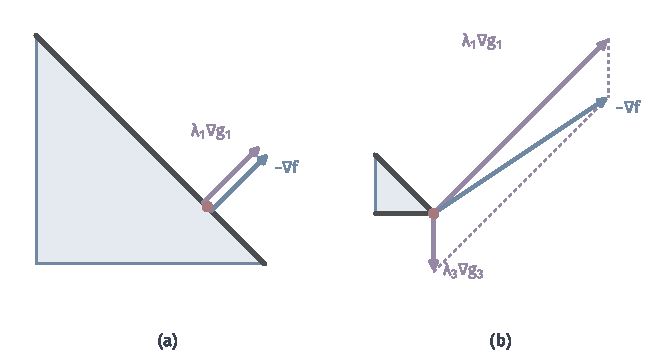
\includegraphics[width=112mm]{figures/05-optimization/06-constrained-optimization/matplotlib/kkt-force-balance/figure.pdf}
  \caption{最优点处的力的平衡。蓝色箭头是负梯度，紫色箭头是$\lambda_i\nabla g_i$。(a)$\tau=2$：$-\nabla f=\frac12\nabla g_1$（两箭头实际重合，为看清而错开绘制）。(b)$\tau=1/2$：$-\nabla f=\frac32\nabla g_1+\frac12\nabla g_3$，虚线组成平行四边形。}
  \label{fig:kkt-force-balance}
\end{BookInlineFigure}

\paragraph{从无下降方向到乘子}
力的平衡是直观，严格的推导要用第~\ref{chap:linear-programming}章的Farkas引理：对矩阵$\bm{M}$和向量$\bm{b}$，系统$\bm{M}\bm{u}=\bm{b}$，$\bm{u}\geq\bm{0}$与系统$\bm{M}^\top\bm{z}\geq\bm{0}$，$\bm{b}^\top\bm{z}<0$恰有一个有解。几何上，$\bm{b}$要么在$\bm{M}$的列张成的锥内，要么能被一个超平面与锥隔开。

\begin{lemma}[无线性化下降方向与乘子]
\label{lem:kkt-farkas}
设$\bar{\bm{x}}\in\bm{C}$，$f$与约束函数在$\bar{\bm{x}}$处可微。不存在$\bm{d}\in\bm{F}(\bar{\bm{x}})$使$\langle\nabla f(\bar{\bm{x}}),\bm{d}\rangle<0$，当且仅当存在$\lambda_i\geq0$（$i\in A(\bar{\bm{x}})$）和$\nu_j\in\mathbb{R}$，使
\begin{equation}
 \nabla f(\bar{\bm{x}})+\sum_{i\in A(\bar{\bm{x}})}\lambda_i\nabla g_i(\bar{\bm{x}})+\sum_{j=1}^p\nu_j\nabla h_j(\bar{\bm{x}})=\bm{0}.
 \label{eq:kkt-farkas-stationary}
\end{equation}
\end{lemma}

\begin{proof}
以活动的$\nabla g_i(\bar{\bm{x}})^\top$为行组成$\bm{B}$，以$\nabla h_j(\bar{\bm{x}})^\top$为行组成$\bm{E}$，在Farkas引理中取
\[
 \bm{M}=\begin{bmatrix}\bm{B}^\top&\bm{E}^\top&-\bm{E}^\top\end{bmatrix},\qquad\bm{b}=-\nabla f(\bar{\bm{x}}).
\]
把等式乘子拆成$\bm{\nu}=\bm{\nu}^{+}-\bm{\nu}^{-}$，两部分都非负，并记
\[
 \bm{u}=(\bm{\lambda}_A,\bm{\nu}^{+},\bm{\nu}^{-})\geq\bm{0},
\]
其中$\bm{\lambda}_A$是活动约束的乘子。方程$\bm{M}\bm{u}=\bm{b}$正是式~\eqref{eq:kkt-farkas-stationary}。

另一个系统要求$\bm{B}\bm{z}\geq\bm{0}$，$\bm{E}\bm{z}=\bm{0}$，$\langle\nabla f(\bar{\bm{x}}),\bm{z}\rangle>0$。令$\bm{d}=-\bm{z}$，它等价于
\[
 \bm{B}\bm{d}\leq\bm{0},\qquad\bm{E}\bm{d}=\bm{0},\qquad\langle\nabla f(\bar{\bm{x}}),\bm{d}\rangle<0,
\]
即存在线性化下降方向。Farkas引理说两个系统恰有一个有解，这就是要证的等价。
\end{proof}

图~\ref{fig:kkt-farkas-cone}画出引理的两种情形，两张图的约束梯度相同。(a)是$\tau=1/2$的角点，$-\nabla f$落在紫色的梯度锥内，乘子存在，绿色的线性化锥与它成钝角，没有下降方向。(b)是$\tau=2$时的角点$(2,0)$，这一点可行但不是最优点。这里$-\nabla f=(0,1)$在锥外。

解驻定方程$(0,-1)+\lambda_1(1,1)+\lambda_3(0,-1)=\bm{0}$，得$\lambda_1=0$，$\lambda_3=-1$，符号不对。负乘子正好指出了下降方向$\bm{d}=(-1,1)$，也就是离开$x_2=0$这堵墙：
\[
 f(2-s,s)=\frac12\bigl[s^2+(1-s)^2\bigr],\qquad\frac{\mathrm{d}}{\mathrm{d}s}f\Big|_{s=0}=-1<0.
\]

\begin{BookInlineFigure}
  \centering
  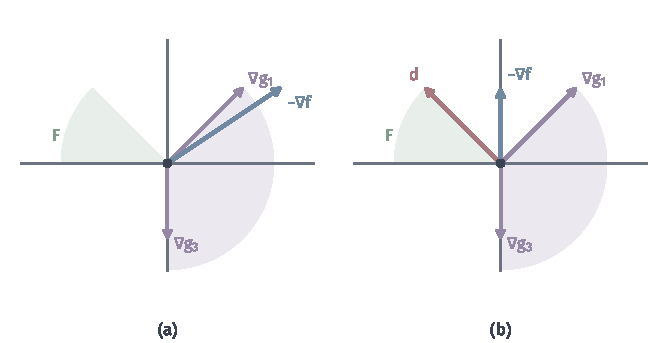
\includegraphics[width=112mm]{figures/05-optimization/06-constrained-optimization/matplotlib/kkt-farkas-cone/figure.pdf}
  \caption{Farkas引理的两种情形，画在方向空间中。紫色楔形是活动梯度张成的锥，浅绿楔形是线性化锥$\bm{F}$，蓝色箭头是$-\nabla f$。(a)$\tau=1/2$的角点：$-\nabla f=(3/2,1)$在锥内。(b)$\tau=2$的角点$(2,0)$：$-\nabla f=(0,1)$在锥外，红色箭头$\bm{d}=(-1,1)$在$\bm{F}$内，与负梯度成锐角，是下降方向。}
  \label{fig:kkt-farkas-cone}
\end{BookInlineFigure}

\paragraph{KKT条件}
式~\eqref{eq:kkt-farkas-stationary}只对活动约束求和。为了不必事先知道哪些约束活动，给每个不等式都配一个乘子，定义完整的Lagrange函数
\begin{equation}
 \mathcal{L}(\bm{x},\bm{\lambda},\bm{\nu})=f(\bm{x})+\sum_{i=1}^m\lambda_ig_i(\bm{x})+\sum_{j=1}^p\nu_jh_j(\bm{x}),
 \label{eq:kkt-lagrangian}
\end{equation}
并用乘积$\lambda_ig_i=0$规定“不活动的约束乘子为零”。这样就得到下面四组条件。

\begin{definition}[KKT条件]
\label{def:kkt-conditions}
设$f$、$g_i$、$h_j$在$\bm{x}^\star$处可微。若存在$\bm{\lambda}^\star\in\mathbb{R}^m$、$\bm{\nu}^\star\in\mathbb{R}^p$，使
\begin{align}
 &\nabla_{\bm{x}}\mathcal{L}(\bm{x}^\star,\bm{\lambda}^\star,\bm{\nu}^\star)=\bm{0}, \label{eq:kkt-stationarity}\\
 &g_i(\bm{x}^\star)\leq0,\quad h_j(\bm{x}^\star)=0, \label{eq:kkt-primal}\\
 &\lambda_i^\star\geq0, \label{eq:kkt-dual}\\
 &\lambda_i^\star g_i(\bm{x}^\star)=0, \label{eq:kkt-complementarity}
\end{align}
对所有$i=1,\ldots,m$，$j=1,\ldots,p$成立，就称$\bm{x}^\star$满足\term{KKT条件}（Karush--Kuhn--Tucker conditions），$(\bm{x}^\star,\bm{\lambda}^\star,\bm{\nu}^\star)$称为\term{KKT点}（KKT point），$(\bm{\lambda}^\star,\bm{\nu}^\star)$称为KKT乘子。
\end{definition}

表~\ref{tab:kkt-four-conditions}列出四组条件的分工。其中式~\eqref{eq:kkt-complementarity}称为互补松弛，它把活动集的选择藏进了乘积里。

\begin{BookInlineTable}
  \centering
  \begin{tabular}{@{}lll@{}}
    \toprule
    条件 & 式子 & 作用\\
    \midrule
    驻定 & \eqref{eq:kkt-stationarity} & 负梯度被约束的法向组合抵消\\
    原始可行 & \eqref{eq:kkt-primal} & 候选点满足全部约束\\
    乘子非负 & \eqref{eq:kkt-dual} & 墙只能推不能拉\\
    互补松弛 & \eqref{eq:kkt-complementarity} & 不活动约束不出力\\
    \bottomrule
  \end{tabular}
  \caption{KKT条件的四个组成部分。}
  \label{tab:kkt-four-conditions}
\end{BookInlineTable}

\paragraph{预算例的计算}
互补松弛把求解变成对活动集的枚举：猜一个活动集，令其余乘子为零，解方程，再检查可行性和符号。预算例的驻定条件是
\[
 x_1-2+\lambda_1-\lambda_2=0,\qquad x_2-1+\lambda_1-\lambda_3=0.
\]

取$\tau=2$。先猜没有活动约束，三个乘子都是零，得$\bm{x}=(2,1)$，但$g_1=1>0$，不可行。再猜只有$g_1$活动，$\lambda_2=\lambda_3=0$，$x_1+x_2=2$，由驻定条件得$x_1=2-\lambda_1$，$x_2=1-\lambda_1$，代入得
\[
 3-2\lambda_1=2,\qquad\lambda_1=\frac12,\qquad\bm{x}=\Bigl(\frac32,\frac12\Bigr).
\]
这一点可行，乘子非负，KKT条件全部成立。

取$\tau=1/2$。只有$g_1$活动时解出$\lambda_1=5/4$，$\bm{x}=(3/4,-1/4)$，不可行。再猜$g_1,g_3$活动，$x_2=0$，$x_1=1/2$，由第一个驻定方程得$\lambda_1=3/2$，第二个得$\lambda_3=\lambda_1-1=1/2$。全部条件成立。

让$\tau$连续变化，结果分三段：
\begin{equation}
 (\bm{x}^\star,\lambda_1,\lambda_3)=\begin{cases}
 \bigl((\tau,0),\ 2-\tau,\ 1-\tau\bigr),&0<\tau\leq1,\\
 \bigl((\tfrac{1+\tau}{2},\tfrac{\tau-1}{2}),\ \tfrac{3-\tau}{2},\ 0\bigr),&1\leq\tau\leq3,\\
 \bigl((2,1),\ 0,\ 0\bigr),&\tau\geq3,
 \end{cases}
 \label{eq:kkt-budget-solution}
\end{equation}
三段都有$\lambda_2=0$。图~\ref{fig:kkt-tau-regimes}画出最优点的轨迹和乘子曲线。

\begin{BookInlineFigure}
  \centering
  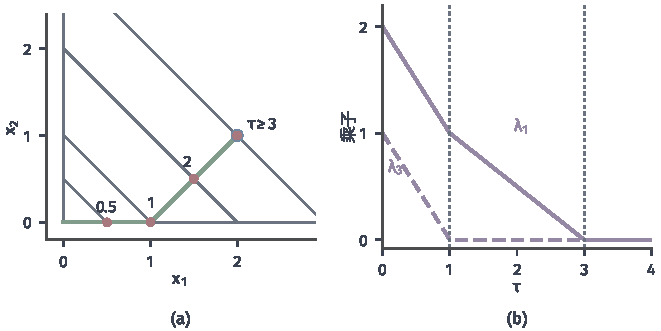
\includegraphics[width=112mm]{figures/05-optimization/06-constrained-optimization/matplotlib/kkt-tau-regimes/figure.pdf}
  \caption{预算例的解随$\tau$变化。(a)绿线是最优点轨迹，深灰细线是预算线$x_1+x_2=\tau$，红点对应$\tau=0.5,1,2,3$，空心点是$\bm{c}$。(b)乘子$\lambda_1$（实线）与$\lambda_3$（虚线），竖直虚线是活动集改变的位置$\tau=1,3$。}
  \label{fig:kkt-tau-regimes}
\end{BookInlineFigure}

这个例子说清了互补松弛的方向。$\lambda_i>0$推出约束活动，但约束活动推不出$\lambda_i>0$。$\tau=3$时预算线恰好经过$\bm{c}$，$g_1$活动，而$\lambda_1=0$：预算恰好够用，这堵墙碰到了点却不用出力。$\tau=1$时最优点是角点$(1,0)$，$g_3$活动，$\lambda_3=0$，同样如此。

从公式~\eqref{eq:kkt-budget-solution}还能再次看到影子价格。$1\leq\tau\leq3$时最优值是$(3-\tau)^2/4$，它对$\tau$的导数是$-(3-\tau)/2=-\lambda_1$：多一块钱，目标改善$\lambda_1$。

\subsection{乘子的存在与唯一性}
\label{sec:kkt-existence}

前面的推导把各步准备好了，现在把它们合起来。

\begin{theorem}[KKT条件的必要性]
\label{thm:kkt-necessary}
设$f$、$g_i$、$h_j$在局部最小点$\bm{x}^\star$附近连续可微。若$\bm{x}^\star$满足MFCQ，则存在KKT乘子$(\bm{\lambda}^\star,\bm{\nu}^\star)$，并且全体KKT乘子组成有界集合。若$\bm{x}^\star$满足LICQ，则KKT乘子唯一。
\end{theorem}

\begin{proof}
\emph{存在性。}由定理~\ref{thm:kkt-mfcq-exact}，切锥等于线性化锥。由定理~\ref{thm:kkt-tangent-necessary}，$\bm{F}(\bm{x}^\star)$中没有使$\langle\nabla f(\bm{x}^\star),\bm{d}\rangle<0$的方向。引理~\ref{lem:kkt-farkas}给出活动约束的乘子与$\bm{\nu}^\star$。不活动约束的乘子取零，四组条件全部成立。

\emph{有界性。}若乘子列$(\bm{\lambda}^{(k)},\bm{\nu}^{(k)})$的范数趋于无穷，把驻定方程除以这个范数，取收敛子列，极限$(\bar{\bm{\lambda}},\bar{\bm{\nu}})$的范数为$1$，满足$\bar{\bm{\lambda}}\geq\bm{0}$，不活动分量为零，并且
\[
 \sum_{i\in A(\bm{x}^\star)}\bar{\lambda}_i\nabla g_i(\bm{x}^\star)+\sum_{j=1}^p\bar{\nu}_j\nabla h_j(\bm{x}^\star)=\bm{0}.
\]

把上式与MFCQ的方向$\bar{\bm{d}}$作内积，等式项消失，得到
\[
 \sum_{i\in A(\bm{x}^\star)}\bar{\lambda}_i\langle\nabla g_i(\bm{x}^\star),\bar{\bm{d}}\rangle=0.
\]
每项都非正，而内积严格为负，所以$\bar{\bm{\lambda}}=\bm{0}$。剩下的等式项由$\nabla h_j$线性无关推出$\bar{\bm{\nu}}=\bm{0}$，与范数为$1$矛盾。

\emph{唯一性。}设有两组KKT乘子。不活动分量都是零，两个驻定方程相减，得到活动梯度和等式梯度的一个线性组合等于零，系数是两组乘子之差。LICQ说明系数全为零。
\end{proof}

由引理~\ref{lem:kkt-licq-implies-mfcq}，LICQ下存在性自动成立。全部活动约束与等式约束都是仿射函数时，$\bm{T}_{\bm{C}}=\bm{F}$不需要任何资格，乘子同样存在，只是有界性和唯一性不再有保证。

\paragraph{存在与唯一是两回事}
图~\ref{fig:kkt-multiplier-sets}对比几种情形的乘子集合。把预算线写两遍（$\tau=2$），MFCQ成立，驻定条件只约束$\lambda_1+\lambda_1'$的和，$\lambda_1+\lambda_1'=1/2$是一条线段：乘子存在、有界，但不唯一。

再看在$\{0\}$上最小化$x$。写成$x\leq0$，$-x\leq0$时，驻定方程是$1+\lambda_1-\lambda_2=0$，解集是无界射线，MFCQ不成立时有界性确实可能失去。写成$x=0$时，$\nu=-1$是唯一乘子。

\paragraph{没有乘子的最小点}
第三种写法最值得注意。最小化$x$，约束$g(x)=x^2\leq0$。可行集只有原点，所以$x^\star=0$是全局最小点。驻定方程是
\[
 1+\lambda\cdot2x^\star=1=0,
\]
对任何$\lambda$都无解，图~\ref{fig:kkt-multiplier-sets}(c)的残差恒为$1$。这是一个没有KKT乘子的最小点。

因此，不能仅凭驻定方程无解就排除一个候选点，除非已经确认它满足约束资格。这里的问题出在约束函数的写法上，$\nabla g(0)=0$让约束的一阶信息完全失效，与目标函数无关。

\begin{BookInlineFigure}
  \centering
  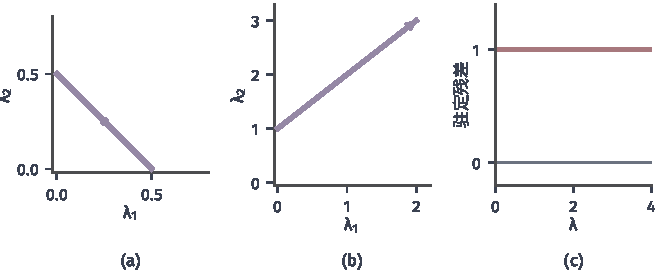
\includegraphics[width=112mm]{figures/05-optimization/06-constrained-optimization/matplotlib/kkt-multiplier-sets/figure.pdf}
  \caption{KKT乘子集合的三种情况。(a)预算线写两遍（$\tau=2$），乘子集合是线段$\lambda_1+\lambda_2=1/2$（这里$\lambda_2$表示重复约束的乘子），有界而不唯一。(b)$\min x$，约束$x\leq0$，$-x\leq0$：乘子集合是无界射线$\lambda_2=1+\lambda_1$。(c)$\min x$，约束$x^2\leq0$：对任何乘子，驻定残差都等于$1$，乘子不存在。}
  \label{fig:kkt-multiplier-sets}
\end{BookInlineFigure}

\subsection{凸问题的全局判别}
\label{sec:kkt-convex}

KKT条件在约束资格下是必要的，它能筛掉不合格的点，却不能确认合格的点就是最小点。什么时候能反过来？答案是问题凸的时候，而且这时连约束资格都不用检查。

\begin{theorem}[凸问题的KKT充分性]
\label{thm:kkt-convex-sufficient}
设$\bm{D}\subseteq\mathbb{R}^n$是包含可行集的开凸集，$f$与$g_i$在$\bm{D}$上凸且可微，$h_j$是仿射函数。若$(\bm{x}^\star,\bm{\lambda}^\star,\bm{\nu}^\star)$是KKT点，则$\bm{x}^\star$是问题~\eqref{eq:kkt-problem}的全局最小点。
\end{theorem}

\begin{proof}
任取可行点$\bm{x}$，记$\bm{u}=\bm{x}-\bm{x}^\star$。由第~\ref{chap:optimization}章的一阶支撑不等式，凸函数$f$满足
\[
 f(\bm{x})\geq f(\bm{x}^\star)+\langle\nabla f(\bm{x}^\star),\bm{u}\rangle.
\]
再由驻定条件~\eqref{eq:kkt-stationarity}，把梯度替换掉：
\[
 f(\bm{x})\geq f(\bm{x}^\star)-\sum_{i=1}^m\lambda_i^\star\langle\nabla g_i(\bm{x}^\star),\bm{u}\rangle-\sum_{j=1}^p\nu_j^\star\langle\nabla h_j(\bm{x}^\star),\bm{u}\rangle.
\]

$h_j$仿射，$\bm{x}$与$\bm{x}^\star$都可行，所以
\[
 \langle\nabla h_j(\bm{x}^\star),\bm{u}\rangle=h_j(\bm{x})-h_j(\bm{x}^\star)=0,
\]
最后一个和式消失。

对$\lambda_i^\star=0$的项，这一项本来就是零。对$\lambda_i^\star>0$的项，互补松弛给出$g_i(\bm{x}^\star)=0$，再对凸函数$g_i$用支撑不等式：
\[
 \langle\nabla g_i(\bm{x}^\star),\bm{u}\rangle\leq g_i(\bm{x})-g_i(\bm{x}^\star)=g_i(\bm{x})\leq0.
\]
所以和式中每一项$-\lambda_i^\star\langle\nabla g_i,\bm{u}\rangle$都非负，代回得到$f(\bm{x})\geq f(\bm{x}^\star)$。
\end{proof}

证明的每一步都用到了相应的假设：目标凸给出一个全局下界，$g_i$凸把梯度内积换成函数值，乘子非负保证不等号的方向，互补松弛消去$g_i(\bm{x}^\star)$，等式仿射让等式项消失。

把它用在预算例上。目标凸，约束都是仿射函数，所以式~\eqref{eq:kkt-budget-solution}中的点都是全局最小点，这一步不需要再检查什么。

还可以从Lagrange函数看这个结论。固定乘子后，$\mathcal{L}(\cdot,\bm{\lambda}^\star,\bm{\nu}^\star)$是凸函数，驻定点就是它的全局最小点。在可行点上$\mathcal{L}\leq f$，在$\bm{x}^\star$处两者相等，于是目标在$\bm{x}^\star$被一个碗从下面托住了。图~\ref{fig:kkt-convex-vs-nonconvex}(a)取最小化$(x-2)^2$、约束$x-1\leq0$的问题，$x^\star=1$，$\lambda^\star=2$，$\mathcal{L}(x,2)=(x-1)^2+1$就是紫色的碗，可行域上它在$f$的下方。

\begin{BookInlineFigure}
  \centering
  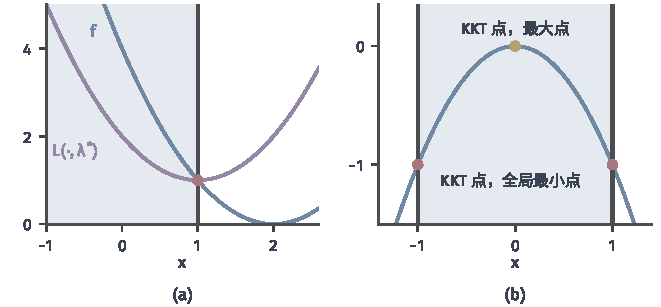
\includegraphics[width=112mm]{figures/05-optimization/06-constrained-optimization/matplotlib/kkt-convex-vs-nonconvex/figure.pdf}
  \caption{凸与非凸问题中的KKT点。浅蓝带是可行域，深灰线是活动约束的位置。(a)$\min(x-2)^2$，$x\leq1$：KKT点$x^\star=1$（红），$\lambda^\star=2$。紫色曲线$\mathcal{L}(x,2)=(x-1)^2+1$在可行域上位于$f$（蓝）下方，并在$x^\star$处与$f$相接。(b)$\min-x^2$，$\lvert x\rvert\leq1$：三个KKT点中$x=0$（黄）是最大点，$x=\pm1$（红）是全局最小点。}
  \label{fig:kkt-convex-vs-nonconvex}
\end{BookInlineFigure}

\paragraph{去掉凸性会怎样}
一般非凸问题中，KKT条件只提供候选。在$[-1,1]$上最小化$-x^2$，约束写成$x-1\leq0$，$-x-1\leq0$。点$x=0$没有活动约束，$f'(0)=0$，乘子取零就满足KKT条件，但它是全局最大点。点$x=1$处由$-2+\lambda_1=0$得$\lambda_1=2$，也满足KKT条件，它才是最小点。KKT方程分不开这两种点，见图~\ref{fig:kkt-convex-vs-nonconvex}(b)。

等式必须是仿射函数也不是多余的要求。单位圆周的$h(\bm{x})=x_1^2+x_2^2-1$是凸函数，目标$\frac12\lVert\bm{x}-(2,0)\rVert_2^2$也是凸函数，但$(-1,0)$是KKT点，却是圆周上的全局最大点。$h=0$的解集不是凸集，定理的证明在处理等式项那一步就失效了。

另外，充分性不提供存在性。$\min x$，$x^2\leq0$是凸问题，最小点却没有KKT乘子。表~\ref{tab:kkt-necessity-sufficiency}把必要性与充分性的条件放在一起。

\begin{BookInlineTable}
  \centering
  \begin{tabular}{@{}lll@{}}
    \toprule
    结论方向 & 所需条件 & 结论\\
    \midrule
    局部最小$\Rightarrow$KKT & MFCQ（或LICQ、仿射约束） & 存在乘子\\
    KKT$\Rightarrow$全局最小 & 目标、$g_i$凸，$h_j$仿射 & 不需要约束资格\\
    KKT$\Rightarrow$局部最小 & 一般不成立 & 需要二阶条件\\
    \bottomrule
  \end{tabular}
  \caption{KKT条件的必要性与充分性。}
  \label{tab:kkt-necessity-sufficiency}
\end{BookInlineTable}

\section{二阶条件}
\label{sec:kkt-second-order}

KKT点可能是最小点，也可能不是。单位圆周上最小化$\frac12\lVert\bm{x}-(2,0)\rVert_2^2$就是例子：离$(2,0)$最近和最远的点都满足一阶条件。这就需要回答：一阶信息判断不了的时候，曲率怎样作出判断？这需要先确定该检查哪些方向，再确定该检查谁的曲率。

\subsection{临界锥}
\label{sec:kkt-critical-cone}

设$(\bm{x}^\star,\bm{\lambda}^\star,\bm{\nu}^\star)$是KKT点。对线性化方向$\bm{d}\in\bm{F}(\bm{x}^\star)$，由驻定条件，目标的一阶变化是
\[
 \langle\nabla f(\bm{x}^\star),\bm{d}\rangle=-\sum_{i\in A(\bm{x}^\star)}\lambda_i^\star\langle\nabla g_i(\bm{x}^\star),\bm{d}\rangle-\sum_{j=1}^p\nu_j^\star\langle\nabla h_j(\bm{x}^\star),\bm{d}\rangle.
\]
等式项为零。每个$\lambda_i^\star\geq0$，每个$\langle\nabla g_i,\bm{d}\rangle\leq0$，所以右端是非负项之和。

若这个值严格为正，目标沿$\bm{d}$一阶上升，这个方向已经判决完毕，二阶项不用看。需要继续检查的，只有一阶变化恰好为零的方向。一个非负项之和为零，当且仅当每一项为零，所以这些方向在$\lambda_i^\star>0$的活动约束上必须取等号。

\begin{definition}[临界锥]
\label{def:kkt-critical-cone}
设$(\bm{x}^\star,\bm{\lambda}^\star,\bm{\nu}^\star)$是KKT点。集合
\begin{equation}
 \bm{K}(\bm{x}^\star,\bm{\lambda}^\star)=\left\{\bm{d}\in\bm{F}(\bm{x}^\star):
 \langle\nabla g_i(\bm{x}^\star),\bm{d}\rangle=0\ \text{对所有}\ \lambda_i^\star>0
 \right\}
 \label{eq:kkt-critical-cone}
\end{equation}
称为\term{临界锥}（critical cone）。由上面的推导，它等于
\begin{equation}
 \bm{K}(\bm{x}^\star,\bm{\lambda}^\star)=\{\bm{d}\in\bm{F}(\bm{x}^\star):\langle\nabla f(\bm{x}^\star),\bm{d}\rangle=0\}.
 \label{eq:kkt-critical-cone-f}
\end{equation}
\end{definition}

式~\eqref{eq:kkt-critical-cone-f}的右端不含乘子，所以即使乘子不唯一，临界锥也不依赖乘子的选择。两种写法各有用处：式~\eqref{eq:kkt-critical-cone}便于计算，式~\eqref{eq:kkt-critical-cone-f}说明它的含义。

零乘子的活动约束值得单独看。这样的约束在式~\eqref{eq:kkt-critical-cone}里没有被要求取等号，它仍然保留$\langle\nabla g_i,\bm{d}\rangle\leq0$的单侧限制。所以临界锥一般是锥，不是子空间。

用预算例算三种情况，见图~\ref{fig:kkt-critical-cone}。$\tau=1/2$的角点，$\lambda_1,\lambda_3$都为正，两条约束都取等号，$d_1+d_2=0$，$d_2=0$，于是$\bm{K}=\{\bm{0}\}$：一阶条件已经判决了所有方向。

$\tau=1$的角点$(1,0)$，$\lambda_1=1>0$，$\lambda_3=0$，于是$g_1$取等号，$g_3$只保留单侧：
\[
 \bm{K}=\{\bm{d}:d_1+d_2=0,\ d_2\geq0\}=\{s(-1,1):s\geq0\}.
\]
沿预算线向上走的这一条射线，一阶变化为零，要靠二阶项判断。而反方向$(1,-1)$不可行。

\begin{BookInlineFigure}
  \centering
  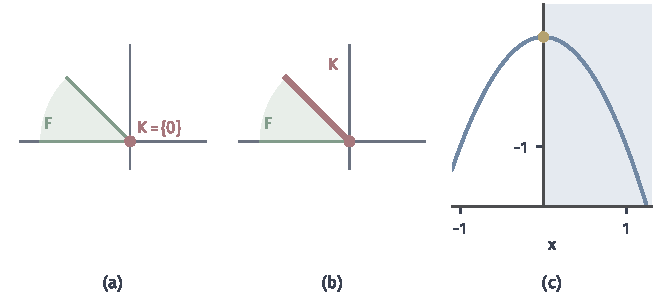
\includegraphics[width=112mm]{figures/05-optimization/06-constrained-optimization/matplotlib/kkt-critical-cone/figure.pdf}
  \caption{临界锥（红色）与线性化锥$\bm{F}$（绿色）。(a)预算例$\tau=1/2$的角点，两个乘子都为正，$\bm{K}=\{\bm{0}\}$。(b)预算例$\tau=1$的角点，$\lambda_3=0$，$\bm{K}$是射线$s(-1,1)$，$s\geq0$。(c)$\min-x^2$，$x\geq0$（蓝色带），黄点$x=0$是KKT点，乘子为零，$\bm{K}=[0,\infty)$。}
  \label{fig:kkt-critical-cone}
\end{BookInlineFigure}

\paragraph{不能把活动约束都当成等式}
一种常见的简化是把所有活动约束当成等式，对每个活动的$g_i$都要求$\langle\nabla g_i,\bm{d}\rangle=0$。下面的例子说明这样会漏掉下降方向。最小化$f(x)=-x^2$，约束$g(x)=-x\leq0$。在$x=0$处，$f'(0)=0$，所以$\lambda=0$，KKT条件成立。

约束活动而乘子为零，真正的临界锥是$\{d:-d\leq0\}=[0,\infty)$。沿$d=1$，$f''(0)d^2=-2<0$，二阶检验发现$x=0$不是局部最小点，事实上$f(t)=-t^2<0$。

要是把约束当成等式，方向只剩$\{0\}$，就没有方向可供检查，会错误地接受$x=0$。图~\ref{fig:kkt-critical-cone}(c)就是这个例子。

\subsection{二阶必要条件}
\label{sec:kkt-sonc}

下一个问题是该检查谁的曲率。答案不是目标的Hessian，用下面的例子就能看清。

\paragraph{约束的弯曲进入曲率}
在单位圆周上最小化$f(\bm{x})=\frac12[(x_1-2)^2+x_2^2]$，也就是找圆周上离$(2,0)$最近的点。令$h(\bm{x})=x_1^2+x_2^2-1$，驻定条件是
\[
 x_1-2+2\nu x_1=0,\qquad x_2+2\nu x_2=0.
\]
第二式说明$x_2=0$或$\nu=-1/2$。后者代入第一式得$-2=0$，不可能，所以$x_2=0$，$x_1=\pm1$。两个KKT点是
\[
 (1,0),\ \nu=\frac12;\qquad(-1,0),\ \nu=-\frac32.
\]

这两点的目标Hessian都是单位阵，正定，分不开。用角度参数化圆周，目标变成
\[
 \phi(\theta)=f(\cos\theta,\sin\theta)=\frac52-2\cos\theta,\qquad\phi''(\theta)=2\cos\theta.
\]
在$(1,0)$处$\phi''=2$，是极小；在$(-1,0)$处$\phi''=-2$，是极大。图~\ref{fig:kkt-constraint-curvature}(b)的黄色抛物线就是这两个曲率。

\begin{BookInlineFigure}
  \centering
  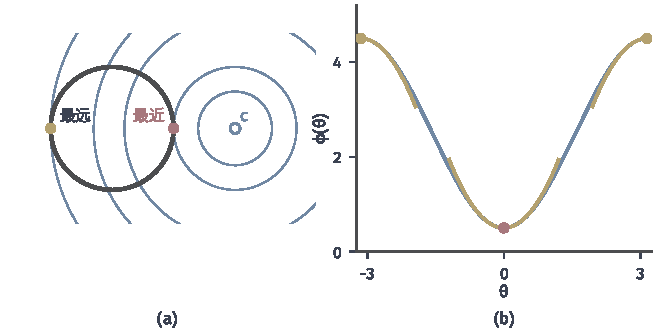
\includegraphics[width=112mm]{figures/05-optimization/06-constrained-optimization/matplotlib/kkt-constraint-curvature/figure.pdf}
  \caption{约束的弯曲改变了有效曲率。(a)深灰圆是可行集，蓝线是目标$\frac12\lVert\bm{x}-\bm{c}\rVert_2^2$（$\bm{c}=(2,0)$）的等高线。红点$(1,0)$是最近点，黄点$(-1,0)$是最远点，两者都是KKT点，目标Hessian都是单位阵。(b)沿圆周的目标值$\phi(\theta)=5/2-2\cos\theta$，黄色抛物线是两点处曲率分别为$2$、$-2$的二次近似。}
  \label{fig:kkt-constraint-curvature}
\end{BookInlineFigure}

这两个数从哪里来？沿可行曲线$\bm{x}(t)$，$\bm{x}(0)=\bm{x}^\star$，$\bm{x}'(0)=\bm{d}$，复合函数求二阶导数得到
\[
 \frac{\mathrm{d}^2}{\mathrm{d}t^2}f(\bm{x}(t))\Big|_{t=0}=\bm{d}^\top\nabla^2f(\bm{x}^\star)\bm{d}+\langle\nabla f(\bm{x}^\star),\bm{x}''(0)\rangle.
\]
第二项是曲线的弯曲$\bm{x}''(0)$贡献的，它是约束带来的，只看目标Hessian看不到这一项。

对恒等式$h(\bm{x}(t))=0$同样求两次导数，得到
\[
 \bm{d}^\top\nabla^2h(\bm{x}^\star)\bm{d}+\langle\nabla h(\bm{x}^\star),\bm{x}''(0)\rangle=0.
\]
再由驻定条件$\nabla f=-\nu\nabla h$，弯曲项可以用约束的Hessian表示：
\[
 \langle\nabla f(\bm{x}^\star),\bm{x}''(0)\rangle=-\nu\langle\nabla h(\bm{x}^\star),\bm{x}''(0)\rangle=\nu\,\bm{d}^\top\nabla^2h(\bm{x}^\star)\bm{d}.
\]

两式合起来，沿曲线的二阶导数恰好是
\[
 \bm{d}^\top\bigl(\nabla^2f(\bm{x}^\star)+\nu\nabla^2h(\bm{x}^\star)\bigr)\bm{d},
\]
括号里是Lagrange函数对$\bm{x}$的Hessian。乘子把约束的弯曲折算成了目标的曲率。在例子中$\nabla^2h=2\bm{I}$，$\bm{d}=(0,1)$，代入$(1,0)$得$1+2\cdot\frac12=2$，代入$(-1,0)$得$1+2\cdot(-\frac32)=-2$，与$\phi''$完全一致。

一般地，把Lagrange函数对$\bm{x}$的Hessian记为
\begin{equation}
 \nabla^2_{\bm{x}\bm{x}}\mathcal{L}(\bm{x},\bm{\lambda},\bm{\nu})=\nabla^2f(\bm{x})+\sum_{i=1}^m\lambda_i\nabla^2g_i(\bm{x})+\sum_{j=1}^p\nu_j\nabla^2h_j(\bm{x}).
 \label{eq:kkt-lagrangian-hessian}
\end{equation}

\begin{theorem}[二阶必要条件]
\label{thm:kkt-sonc}
设$f$、$g_i$、$h_j$在局部最小点$\bm{x}^\star$附近二阶连续可微，$\bm{x}^\star$满足LICQ，$(\bm{\lambda}^\star,\bm{\nu}^\star)$是它唯一的KKT乘子。则
\begin{equation}
 \bm{d}^\top\nabla^2_{\bm{x}\bm{x}}\mathcal{L}(\bm{x}^\star,\bm{\lambda}^\star,\bm{\nu}^\star)\bm{d}\geq0
 \quad\text{对所有}\ \bm{d}\in\bm{K}(\bm{x}^\star,\bm{\lambda}^\star).
 \label{eq:kkt-sonc}
\end{equation}
\end{theorem}

\begin{proof}
取$\bm{d}\in\bm{K}$，令
\[
 W=\{i\in A(\bm{x}^\star):\langle\nabla g_i(\bm{x}^\star),\bm{d}\rangle=0\}.
\]
由临界锥的定义，$\lambda_i^\star>0$的下标都在$W$中。LICQ保证引理~\ref{lem:kkt-feasible-curve}适用，得到二阶连续可微的可行曲线$\bm{x}(t)$，$0\leq t<\delta$，它沿$\bm{d}$出发，并使$h_j$与$g_i$（$i\in W$）恒为零。

令$\phi(t)$是乘子固定为$(\bm{\lambda}^\star,\bm{\nu}^\star)$时Lagrange函数沿曲线的值。曲线上等式约束为零，$i\in W$的约束为零，其余约束的乘子为零，所以对$0\leq t<\delta$，
\[
 \phi(t)=\mathcal{L}(\bm{x}(t),\bm{\lambda}^\star,\bm{\nu}^\star)=f(\bm{x}(t)).
\]
这是使用Lagrange函数的好处：在这条曲线上，它和目标完全一样，但它的梯度在$\bm{x}^\star$处为零。

由驻定条件，
\[
 \phi'(0)=\langle\nabla_{\bm{x}}\mathcal{L}(\bm{x}^\star,\bm{\lambda}^\star,\bm{\nu}^\star),\bm{d}\rangle=0.
\]
再求一次导数，含$\bm{x}''(0)$的项同样因$\nabla_{\bm{x}}\mathcal{L}=\bm{0}$消失，得到
\[
 \phi''(0)=\bm{d}^\top\nabla^2_{\bm{x}\bm{x}}\mathcal{L}(\bm{x}^\star,\bm{\lambda}^\star,\bm{\nu}^\star)\bm{d}.
\]

$\bm{x}(t)$可行且趋于局部最小点，所以小的$t>0$时$\phi(t)\geq\phi(0)$。由Taylor公式，$\phi(t)-\phi(0)=\frac12\phi''(0)t^2+o(t^2)$，除以$t^2$并令$t\downarrow0$，得到$\phi''(0)\geq0$。
\end{proof}

定理中的LICQ负责把每个临界方向实现成可行曲线。没有约束资格时，临界方向可能只是线性化的产物。最小化$-x^2$，约束$x^2\leq0$，原点是唯一可行点，取乘子$\lambda=0$是一组KKT乘子，此时$\nabla^2_{xx}\mathcal{L}=-2$，$\bm{K}=\mathbb{R}$，式~\eqref{eq:kkt-sonc}不成立，而原点当然是最小点。

\paragraph{两种错误的简化}
条件~\eqref{eq:kkt-sonc}既不等同于目标Hessian半正定，也不等同于在全空间半正定。圆周例已经说明目标Hessian可以正定而点不是局部最小点。

反过来，全空间的不定性也不妨碍极小。最小化$x_1^2-x_2^2$，约束$x_2=0$，原点处$\nu=0$，Lagrange Hessian是$\operatorname{diag}(2,-2)$，不定。但临界锥是$\{\bm{d}:d_2=0\}$，上面的二次型是$2d_1^2\geq0$。原点确实是最小点，负曲率的方向被约束禁止了。

\subsection{二阶充分条件}
\label{sec:kkt-sosc}

必要条件是用来排除的，充分条件是用来确认的。把不等号换成严格，就能确认局部最优，并且还能给出增长的速度。值得注意的是，这里不需要约束资格。

\begin{theorem}[二阶充分条件]
\label{thm:kkt-sosc}
设$f$、$g_i$、$h_j$在$\bm{x}^\star$附近二阶连续可微，$(\bm{x}^\star,\bm{\lambda}^\star,\bm{\nu}^\star)$是KKT点，并且
\begin{equation}
 \bm{d}^\top\nabla^2_{\bm{x}\bm{x}}\mathcal{L}(\bm{x}^\star,\bm{\lambda}^\star,\bm{\nu}^\star)\bm{d}>0
 \quad\text{对所有非零}\ \bm{d}\in\bm{K}(\bm{x}^\star,\bm{\lambda}^\star).
 \label{eq:kkt-sosc}
\end{equation}
则存在$\sigma>0$，$r>0$，使
\begin{equation}
 f(\bm{x})\geq f(\bm{x}^\star)+\sigma\lVert\bm{x}-\bm{x}^\star\rVert_2^2
 \quad\text{对所有}\ \bm{x}\in\bm{C},\ \lVert\bm{x}-\bm{x}^\star\rVert_2<r.
 \label{eq:kkt-quadratic-growth}
\end{equation}
特别地，$\bm{x}^\star$是严格局部最小点。
\end{theorem}

\begin{proof}
反设结论不成立。对每个$k$取$\sigma=1/k$，存在可行点$\bm{x}^{(k)}\neq\bm{x}^\star$，$\bm{x}^{(k)}\to\bm{x}^\star$，使
\[
 f(\bm{x}^{(k)})<f(\bm{x}^\star)+\frac1k\lVert\bm{x}^{(k)}-\bm{x}^\star\rVert_2^2.
\]
记$t_k=\lVert\bm{x}^{(k)}-\bm{x}^\star\rVert_2$，$\bm{d}^{(k)}=(\bm{x}^{(k)}-\bm{x}^\star)/t_k$。单位向量列有收敛子列，不妨设$\bm{d}^{(k)}\to\bm{d}$，$\lVert\bm{d}\rVert_2=1$。按定义~\ref{def:kkt-tangent-cone}，$\bm{d}$是切向量，由定理~\ref{thm:kkt-tangent-in-linearized}，$\bm{d}\in\bm{F}(\bm{x}^\star)$。

\emph{第一步：$\bm{d}$是临界方向。}上面的不等式减去$f(\bm{x}^\star)$，除以$t_k$，令$k\to\infty$，得到$\langle\nabla f(\bm{x}^\star),\bm{d}\rangle\leq0$。第~\ref{sec:kkt-critical-cone}节已经证明，$\bm{d}\in\bm{F}$时这个内积是非负项之和，所以它等于零。由式~\eqref{eq:kkt-critical-cone-f}，$\bm{d}\in\bm{K}$。

\emph{第二步：比较Lagrange函数。}下面乘子固定为$(\bm{\lambda}^\star,\bm{\nu}^\star)$，把Lagrange函数简记为$\mathcal{L}(\bm{x})$。$\bm{x}^{(k)}$可行，$\bm{\lambda}^\star\geq\bm{0}$，所以$\mathcal{L}(\bm{x}^{(k)})\leq f(\bm{x}^{(k)})$。由互补松弛和等式约束，$\mathcal{L}(\bm{x}^\star)=f(\bm{x}^\star)$。于是
\[
 \mathcal{L}(\bm{x}^{(k)})-\mathcal{L}(\bm{x}^\star)\leq f(\bm{x}^{(k)})-f(\bm{x}^\star)<\frac{t_k^2}{k}.
\]

\emph{第三步：展开。}在$\bm{x}^\star$处$\nabla_{\bm{x}}\mathcal{L}=\bm{0}$，由二阶Taylor公式，
\[
 \mathcal{L}(\bm{x}^{(k)})-\mathcal{L}(\bm{x}^\star)=\frac{t_k^2}{2}(\bm{d}^{(k)})^\top\nabla^2_{\bm{x}\bm{x}}\mathcal{L}(\bm{x}^\star)\bm{d}^{(k)}+o(t_k^2).
\]
代入上式，除以$t_k^2$，令$k\to\infty$，得到
\[
 \frac12\bm{d}^\top\nabla^2_{\bm{x}\bm{x}}\mathcal{L}(\bm{x}^\star)\bm{d}\leq0.
\]
这与式~\eqref{eq:kkt-sosc}矛盾。
\end{proof}

证明从头到尾没有用到切锥等于线性化锥，只用了$\bm{T}_{\bm{C}}\subseteq\bm{F}$这个总成立的方向，所以不需要约束资格。它也只要求某一组KKT乘子满足式~\eqref{eq:kkt-sosc}。

在圆周的最近点$(1,0)$，$\bm{K}=\{(0,s)\}$，$\nabla^2_{\bm{x}\bm{x}}\mathcal{L}=2\bm{I}$，条件成立。这里增长式可以精确写出。圆周上，
\[
 f(\bm{x})-\frac12=2-2\cos\theta=\lVert\bm{x}-(1,0)\rVert_2^2,
\]
所以$\sigma=1$。

临界锥只有零向量时，条件~\eqref{eq:kkt-sosc}自动成立，这时一阶条件就足以确认严格局部最小。预算例$\tau=1/2$的角点就是这样。

\paragraph{条件的边界}
严格正性不能放松成半正定。图~\ref{fig:kkt-degenerate-curvature}中三个一元函数在原点的二阶导数都是零，临界锥都是全空间，半正定都成立，可是$x^3$和$-x^4$的原点都不是局部最小点。

严格正性也不是必要的。$x^4$的原点是严格局部最小点，二阶导数却是零。所以二阶必要条件和二阶充分条件之间有一条缝，缝里的情形要靠更高阶的信息或问题的特殊结构。

\begin{BookInlineFigure}
  \centering
  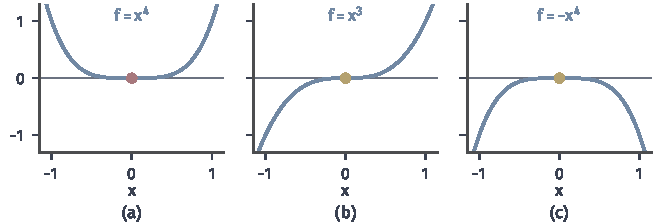
\includegraphics[width=112mm]{figures/05-optimization/06-constrained-optimization/matplotlib/kkt-degenerate-curvature/figure.pdf}
  \caption{二阶导数为零时，二阶条件无法判决。(a)$x^4$：原点（红）是严格局部最小点。(b)$x^3$：原点（黄）不是局部极值点。(c)$-x^4$：原点（黄）是最大点。三者在原点的一、二阶导数都是零。}
  \label{fig:kkt-degenerate-curvature}
\end{BookInlineFigure}

表~\ref{tab:kkt-second-order}对比这两个条件。

\begin{BookInlineTable}
  \centering
  \begin{tabular}{@{}lll@{}}
    \toprule
    对比项 & 二阶必要条件 & 二阶充分条件\\
    \midrule
    出发点 & 已知局部最小点 & 已知KKT点\\
    约束资格 & 需要LICQ & 不需要\\
    二次型 & 在$\bm{K}$上$\geq0$ & 在$\bm{K}$的非零向量上$>0$\\
    结论 & 用于排除候选点 & 严格局部最小，二次增长\\
    \bottomrule
  \end{tabular}
  \caption{二阶必要条件与二阶充分条件的比较。}
  \label{tab:kkt-second-order}
\end{BookInlineTable}

\paragraph{完整走一遍}
最后用一个非凸问题把各项检查串起来：
\begin{equation}
 \min_{\bm{x}\in\mathbb{R}^2}\ -x_1x_2\quad\text{s.t.}\quad g(\bm{x})=x_1^2+x_2^2-2\leq0.
 \label{eq:kkt-full-example}
\end{equation}
可行集是紧的圆盘，目标连续，最小点存在。圆盘内部没有活动约束，边界上$\nabla g=2\bm{x}\neq\bm{0}$，所以LICQ在每个可行点成立，每个局部最小点都满足KKT条件。

驻定条件是
\[
 -x_2+2\lambda x_1=0,\qquad-x_1+2\lambda x_2=0.
\]
由第一式得$x_2=2\lambda x_1$，代入第二式得$x_1=4\lambda^2x_1$。所以要么$x_1=0$，这时$x_2=0$；要么$4\lambda^2=1$。

若$x_1\neq0$，$\lambda=\pm1/2$，都不等于零，互补松弛要求约束活动。$\lambda=1/2$时$x_2=x_1$，代入$g=0$得到$(1,1)$与$(-1,-1)$。$\lambda=-1/2$时$x_2=-x_1$，得到$(1,-1)$与$(-1,1)$，但乘子为负，违反式~\eqref{eq:kkt-dual}，这两点被排除。负乘子说明从这两点沿半径向内走，目标反而下降，这两点其实是最大点。

留下三个KKT点，用二阶条件判决。在原点，$\lambda=0$，$\bm{K}=\mathbb{R}^2$，Hessian和$\bm{d}=(1,1)$给出
\[
 \nabla^2_{\bm{x}\bm{x}}\mathcal{L}=\begin{bmatrix}0&-1\\-1&0\end{bmatrix},\qquad\bm{d}^\top\nabla^2_{\bm{x}\bm{x}}\mathcal{L}\,\bm{d}=-2<0.
\]
原点不满足二阶必要条件，不是局部最小点。

在$(1,1)$，$\lambda=1/2>0$，临界锥要求$\langle\nabla g,\bm{d}\rangle=2d_1+2d_2=0$，即$\bm{d}=s(1,-1)$。Lagrange Hessian是
\[
 \nabla^2_{\bm{x}\bm{x}}\mathcal{L}=\begin{bmatrix}1&-1\\-1&1\end{bmatrix},\qquad\bm{d}^\top\nabla^2_{\bm{x}\bm{x}}\mathcal{L}\,\bm{d}=4s^2>0\ \ (s\neq0).
\]
这个矩阵只是半正定，在$(1,1)$方向为零，但$(1,1)$不是临界方向。二阶充分条件成立，$(1,1)$是严格局部最小点。$(-1,-1)$由对称性相同。

全局最小点存在，又一定在KKT点中。比较目标值，$f(\pm(1,1))=-1$，$f(\bm{0})=0$，所以最优值是$-1$，全局最小点是这两点。这一步用的是“存在性、约束资格、枚举全部候选”这一套全局论证，单靠二阶条件得不到。图~\ref{fig:kkt-full-example}把五个候选点标在一起。

\begin{BookInlineFigure}
  \centering
  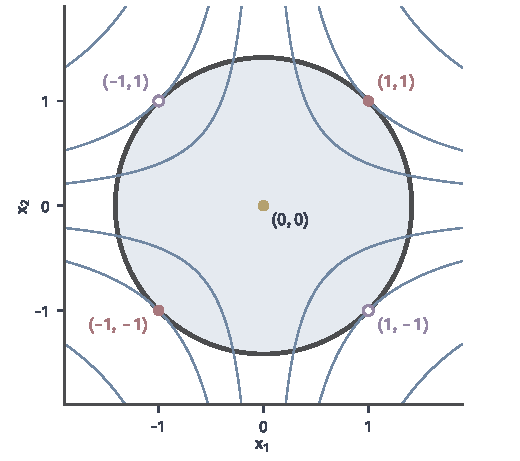
\includegraphics[width=88mm]{figures/05-optimization/06-constrained-optimization/matplotlib/kkt-full-example/figure.pdf}
  \caption{问题~\eqref{eq:kkt-full-example}的候选点。浅蓝圆盘是可行集，蓝线是$-x_1x_2$的等高线。红点$\pm(1,1)$是全局最小点。黄点$(0,0)$是KKT点，但二阶必要条件不成立。紫色空心点$\pm(1,-1)$满足驻定和活动条件，乘子为$-1/2$，不是KKT点。}
  \label{fig:kkt-full-example}
\end{BookInlineFigure}

\section{本章小结}
\label{sec:kkt-summary}

本章回答的问题是：给定一个候选点，怎样只用它附近的信息判断它是否最优。答案不是一个公式，而是按顺序做的几项检查，每一项给出的结论强弱不同，见图~\ref{fig:kkt-decision-flow}。

\begin{BookInlineFigure}
  \centering
  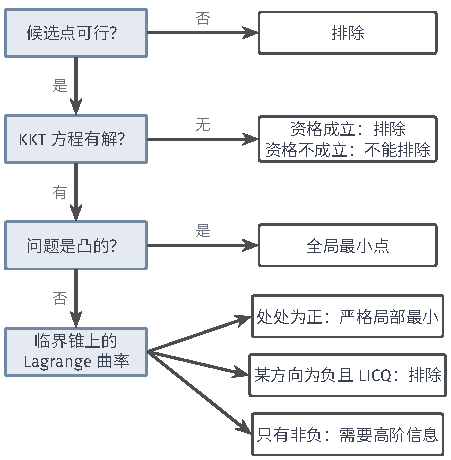
\includegraphics[width=76.3mm]{figures/05-optimization/06-constrained-optimization/tikz/kkt-decision-flow/figure.pdf}
  \caption{判断候选点的流程。左列依次是可行性、KKT方程、凸性和临界锥上的曲率四项检查，右列是对应的结论。“资格”指候选点满足的约束资格，如LICQ或MFCQ。}
  \label{fig:kkt-decision-flow}
\end{BookInlineFigure}

第一项检查是可行性，并找出活动约束。不活动的约束在局部不起作用，所以后面的条件只看活动约束和等式约束。

第二项检查是真实的局部方向。切锥只依赖可行集，它给出最根本的必要条件：局部最小点处，切锥中没有一阶下降方向。线性化锥好算，但可能多出虚假方向。LICQ和MFCQ保证两者相等，这两个条件只涉及约束函数在该点的梯度，与目标的凸性无关，并且会随约束的写法改变。

第三项检查是KKT条件。Farkas引理把“线性化锥中没有下降方向”换成负梯度属于活动梯度的非负锥，由此得到驻定、原始可行、乘子非负和互补松弛四组条件。在MFCQ下它们是局部最小点的必要条件，LICQ进一步保证乘子唯一。没有约束资格时，最小点可以没有乘子。

局部结论和全局结论要分开。目标和不等式约束函数凸、等式约束仿射时，任何KKT点都是全局最小点，这不需要约束资格。一般非凸问题中，KKT点只是候选，全局结论要靠存在性和枚举等其他依据。

第四项检查是曲率。只有一阶变化为零的方向才需要二阶判断，这些方向组成临界锥，零乘子的活动约束在其中保留单侧限制。约束的弯曲通过乘子进入Lagrange函数的Hessian，所以检查的是Lagrange Hessian在临界锥上的二次型，不是目标Hessian，也不是全空间的正定性。LICQ下二次型非负是必要条件；在某组KKT乘子下对非零临界方向严格为正是充分条件，并且给出局部二次增长，这一方向不需要约束资格。两者之间的退化情形，二阶信息判断不了。

这些条件都在已知候选点时做判断，没有回答候选点从哪里来。下一章用乘子构造整个问题的下界，把这里局部的条件变成可以检验的全局证书。可行迭代、乘子更新和局部子问题怎样产生满足这些条件的点，由第~\ref{chap:feasible-iterations}章至第~\ref{chap:nonlinear-interior-point}章研究。

